\documentclass[12pt,a4paper]{article}\usepackage[]{graphicx}\usepackage[]{color}
%% maxwidth is the original width if it is less than linewidth
%% otherwise use linewidth (to make sure the graphics do not exceed the margin)
\makeatletter
\def\maxwidth{ %
  \ifdim\Gin@nat@width>\linewidth
    \linewidth
  \else
    \Gin@nat@width
  \fi
}
\makeatother

\definecolor{fgcolor}{rgb}{0.345, 0.345, 0.345}
\newcommand{\hlnum}[1]{\textcolor[rgb]{0.686,0.059,0.569}{#1}}%
\newcommand{\hlstr}[1]{\textcolor[rgb]{0.192,0.494,0.8}{#1}}%
\newcommand{\hlcom}[1]{\textcolor[rgb]{0.678,0.584,0.686}{\textit{#1}}}%
\newcommand{\hlopt}[1]{\textcolor[rgb]{0,0,0}{#1}}%
\newcommand{\hlstd}[1]{\textcolor[rgb]{0.345,0.345,0.345}{#1}}%
\newcommand{\hlkwa}[1]{\textcolor[rgb]{0.161,0.373,0.58}{\textbf{#1}}}%
\newcommand{\hlkwb}[1]{\textcolor[rgb]{0.69,0.353,0.396}{#1}}%
\newcommand{\hlkwc}[1]{\textcolor[rgb]{0.333,0.667,0.333}{#1}}%
\newcommand{\hlkwd}[1]{\textcolor[rgb]{0.737,0.353,0.396}{\textbf{#1}}}%

\usepackage{framed}
\makeatletter
\newenvironment{kframe}{%
 \def\at@end@of@kframe{}%
 \ifinner\ifhmode%
  \def\at@end@of@kframe{\end{minipage}}%
  \begin{minipage}{\columnwidth}%
 \fi\fi%
 \def\FrameCommand##1{\hskip\@totalleftmargin \hskip-\fboxsep
 \colorbox{shadecolor}{##1}\hskip-\fboxsep
     % There is no \\@totalrightmargin, so:
     \hskip-\linewidth \hskip-\@totalleftmargin \hskip\columnwidth}%
 \MakeFramed {\advance\hsize-\width
   \@totalleftmargin\z@ \linewidth\hsize
   \@setminipage}}%
 {\par\unskip\endMakeFramed%
 \at@end@of@kframe}
\makeatother

\definecolor{shadecolor}{rgb}{.97, .97, .97}
\definecolor{messagecolor}{rgb}{0, 0, 0}
\definecolor{warningcolor}{rgb}{1, 0, 1}
\definecolor{errorcolor}{rgb}{1, 0, 0}
\newenvironment{knitrout}{}{} % an empty environment to be redefined in TeX

\usepackage{alltt}
\usepackage{array}
\usepackage{booktabs}
 \usepackage{amssymb,amsmath,amsthm}
\usepackage[mathscr]{eucal}
\usepackage{calc}
\usepackage{tikz}
\usepackage{courier}
\usepackage{amscd}
\usepackage{verbatim}
\usepackage{mathtools}
\theoremstyle{definition}
\newtheorem{ex}{Exercise}
\usepackage{answers}
\Newassociation{sol}{Solution}{ans}
\usepackage{array}
\usepackage{booktabs}
\usepackage{tikz}
\usetikzlibrary{calc}
\usepackage{dsfont}
\setlength{\parindent}{0cm}



% NUMBERING AND ENVIRONMENTS


%COMMANDS%%%%%%%%%%%%%%%%%%%%%%%%%%%%%%%%%%%%%
\newtheorem{definition}{Definition}
%\newtheorem{theorem}{Theorem}[section]
\newtheorem{theorem}{Theorem}
\newtheorem{lemma}[theorem]{Lemma}
\newtheorem{corollary}[theorem]{Corollary}
\newtheorem{remark}[theorem]{Remark}
\newtheorem{proposition}{Proposition}[section]
\newtheorem{exercise}[theorem]{Exercise}
\newtheorem{problem}[theorem]{Problem}

%IGNORE THESE
\def\mathlexicon#1{$$\vcenter{\halign{\displayandname{##}\hfil&&\qquad
                   \displayandname{##}\hfil\cr #1}}$$}
\def\displayandname#1{\rlap{$\displaystyle\csname
#1\endcsname$}%
                      \qquad \texttt{\char92 #1}}
\IfFileExists{upquote.sty}{\usepackage{upquote}}{}
\begin{document}
\thispagestyle{empty}
\centerline{\bf{Estimating the Average Age of the Williams College Faculty}}
\bigskip
\centerline{By Matt Morris '18}


















\bigskip
My estimated average age for the Williams College Faculty for the last 10 years are as follows:

\begin{center}

2004-2005 = \(45\)

2005-2006 = \(46\)

2006-2007 = \(45.7\)

2007-2008 = \(46.5\)

2008-2009 = \(47\)

2009-2010 = \(48.3\)

2010-2011 = \(48.7\)

2011-2012 = \(48.7\)

2012-2013 = \(48.2\)

2013-2014 = \(48.1\)

\end{center}


\begin{knitrout}
\definecolor{shadecolor}{rgb}{0.969, 0.969, 0.969}\color{fgcolor}
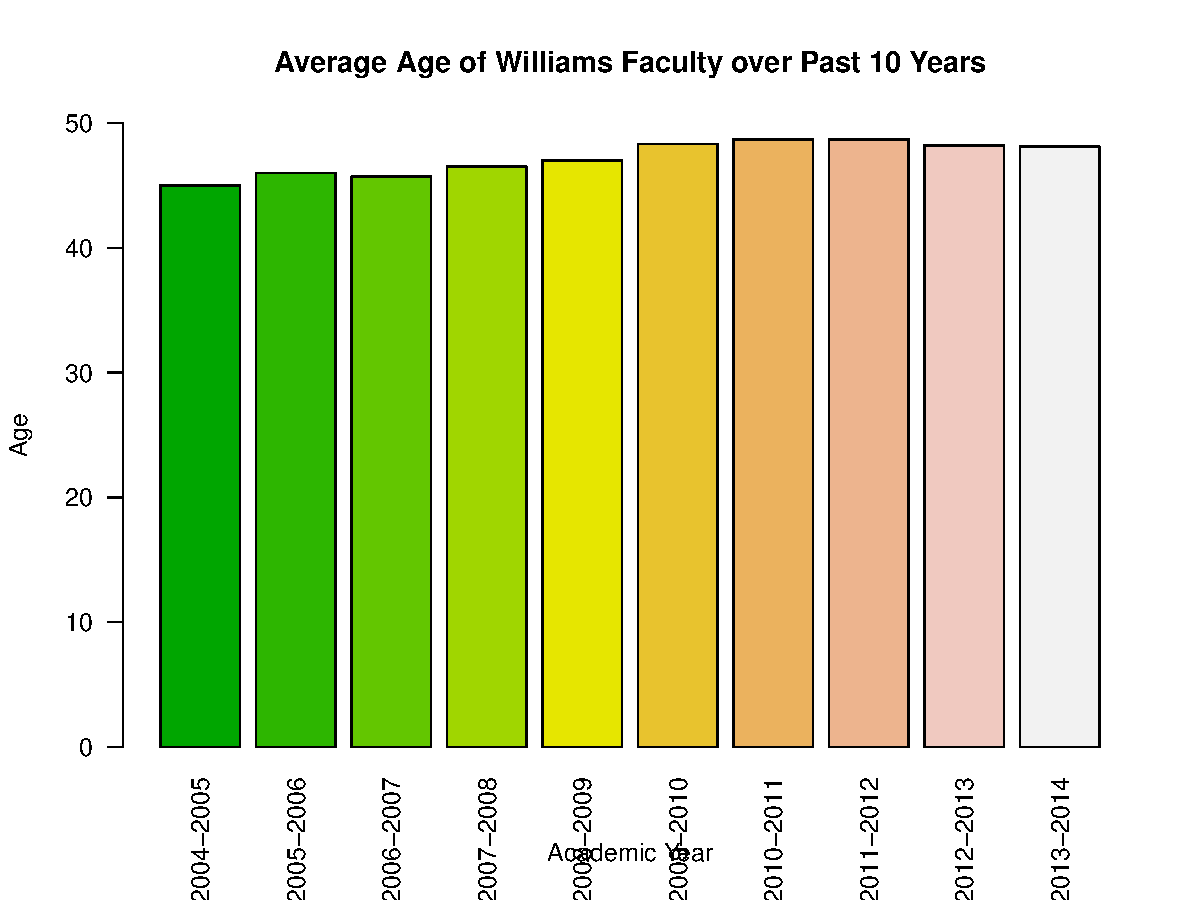
\includegraphics[width=\maxwidth]{figure/unnamed-chunk-6-1} 

\end{knitrout}

\bigskip
Over the last 10 years, the average age of the Williams College Faculty has, on average, increased significantly. Over the last five academic years, while the average age has stagnated around 48, compared to the average age of 45 in the 2004-2005 academic year, a three year increase in average age is important to note.


\bigskip
The youngest and oldest faculty member's age and name for the last 10 years are as follows:

\bigskip
Youngest 2004-2005 = \(24\), Zafrir Levy, Assistant Professor of Physical Education and Head Coach of Men's and Women's Squash

\bigskip
Oldest 2004-2005 = \(83\), Henry J. Bruton, Visiting Professor of Economics

\bigskip
Youngest 2005-2006 = \(25\), Heather N. Harrington, Assistant Project Cataloger

\bigskip
Oldest 2005-2006 = \(84\), Henry J. Bruton, Visting Professor of Economics

\bigskip
Youngest 2006-2007 = \(25\), Robert Michelin, Visting Lecturer in Music and Director of Zambezi

\bigskip
Oldest 2006-2007 = \(85\), Henry J. Bruton Visting Professor of Economics

\bigskip
Youngest 2007-2008 = \(27\), Heather Harrington, Collections Archivist and Marshall K. Creighton, Lecturer in Physical Education

\bigskip
Oldest 2007-2008 = \(86\), Henry J. Bruton, Visting Professor of Economics

\bigskip
Youngest 2008-2009 = \(23\), Binyavanga Wainaina, Sterling Brown '22 Visiting Professor of Africana Studies, First Semester

\bigskip
Oldest 2008-2009 = \(87\), Henry J. Bruton, Visting Professor of Economics

\bigskip
Youngest 2009-2010 = \(26\), David A. Chalifoux, Library Shelving Facility Supervisor

\bigskip
Oldest 2009-2010 = \(88\), Henry J. Bruton, Visting Professor of Economics

\bigskip
Youngest 2010-2011 = \(24\), Daniel Greenberg, Lecturer of Physical Education and Head Men's Tennis Coach

\bigskip
Oldest 2010-2011 = \(89\), Henry J. Bruton, Visting Professor of Economics

\bigskip
Youngest 2011-2012 = \(25\), Daniel Greenberg, Assistant Professor of Physical Education and Head Men's Tennis Coach

\bigskip
Oldest 2011-2012 = \(90\), Henry J. Bruton, Visting Professor of Economics

\bigskip
Youngest 2012-2013 = \(24\), Qing(Wendy) Wang, Assistant Professor of Statistics

\bigskip
Oldest 2012-2013 = \(91\), Henry J. Bruton, Visting Professor of Economics

\bigskip
Youngest 2013-2014 = \(24\), Sarah A. Mirseyedi, Visiting Lecturer in Art

\bigskip
Oldest 2013-2014 = \(77\), Charles B. Dew, Ephraim Williams Professor of American History

\bigskip
How the Number of Faculty have changed over time? Talk about disclaimer about library



\begin{knitrout}
\definecolor{shadecolor}{rgb}{0.969, 0.969, 0.969}\color{fgcolor}
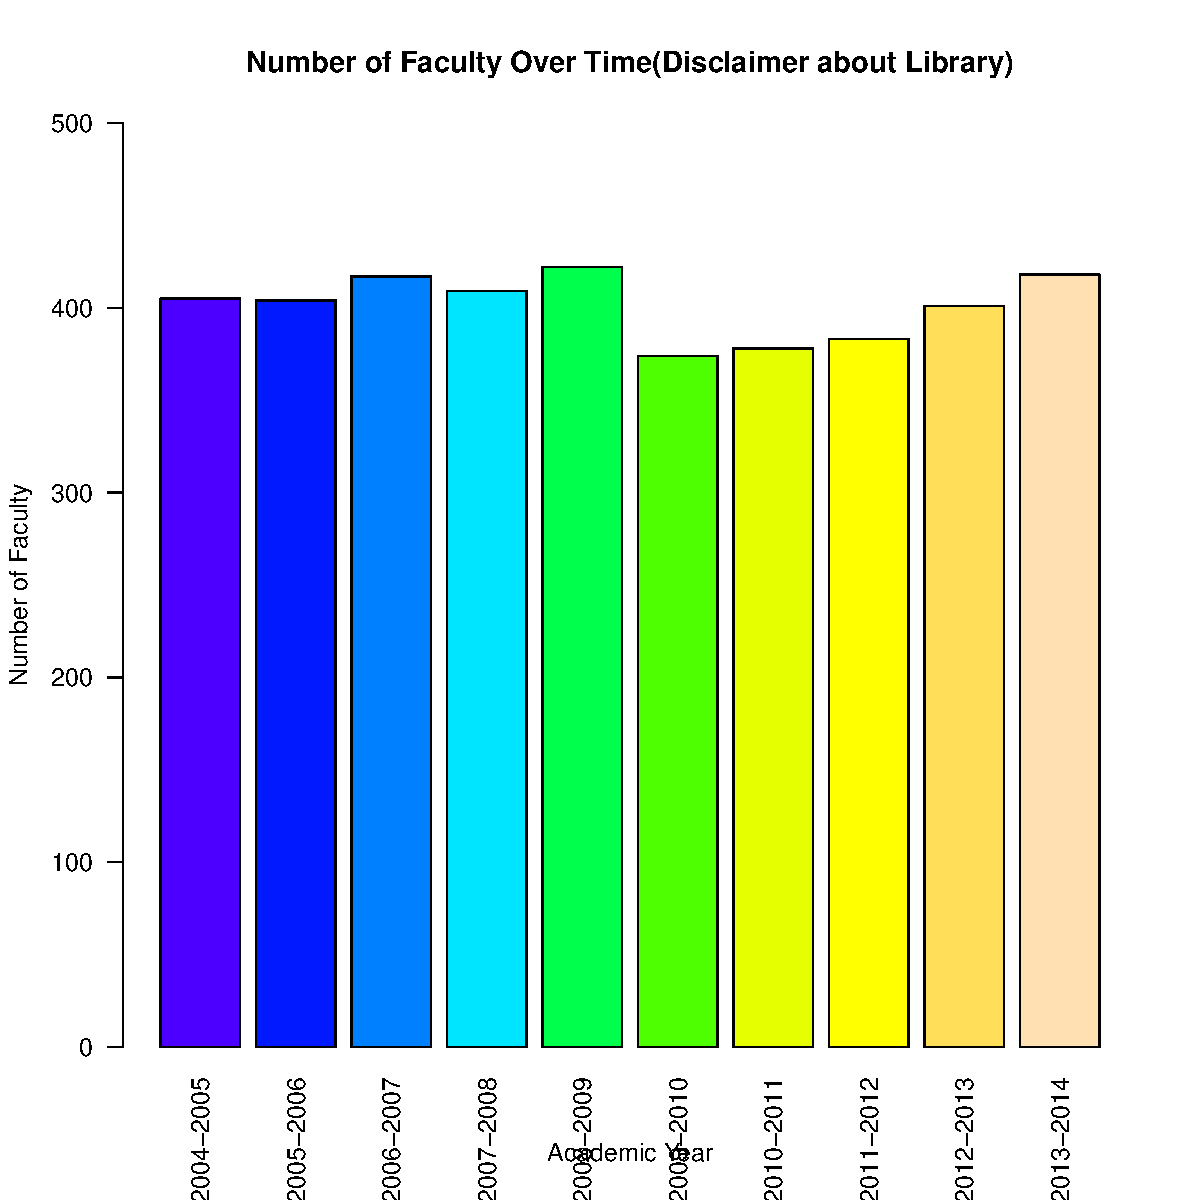
\includegraphics[width=\maxwidth]{figure/unnamed-chunk-8-1} 

\end{knitrout}

\begin{center}
Number of Faculty by Academic Year(LIB Disclaimer)

2004-2005 = 405

2005-2006 = 404

2006-2007 = 417

2007-2008 = 409

2008-2009 = 422

2009-2010 = 374

2010-2011 = 378

2011-2012 = 383

2012-2013 = 401

2013-2014 = 418
\end{center}

\bigskip

While examining the number of faculty by academic year in the last 10 years it appears as though the number of faculty increased somewhat steadily from the 2004-2005 academic year through the 2008-2009 academic year and then dropped off significantly after the 2008-2009 academic year from 422 to 378. This data is somewhat misleading as the Library faculty were only included in the course catalog archives through the 2010-2011 academic year. This suggests that the number of faculty in the last three academic years is most likely about 25 faculty members lower than it actually was. 

\bigskip

A key question in our analysis of the Williams College faculty for the past 10 years is how the age distribution has changed over time. By examining histograms over the last 10 years it is easy to observe the trends in the faculty member ages.

\begin{knitrout}
\definecolor{shadecolor}{rgb}{0.969, 0.969, 0.969}\color{fgcolor}
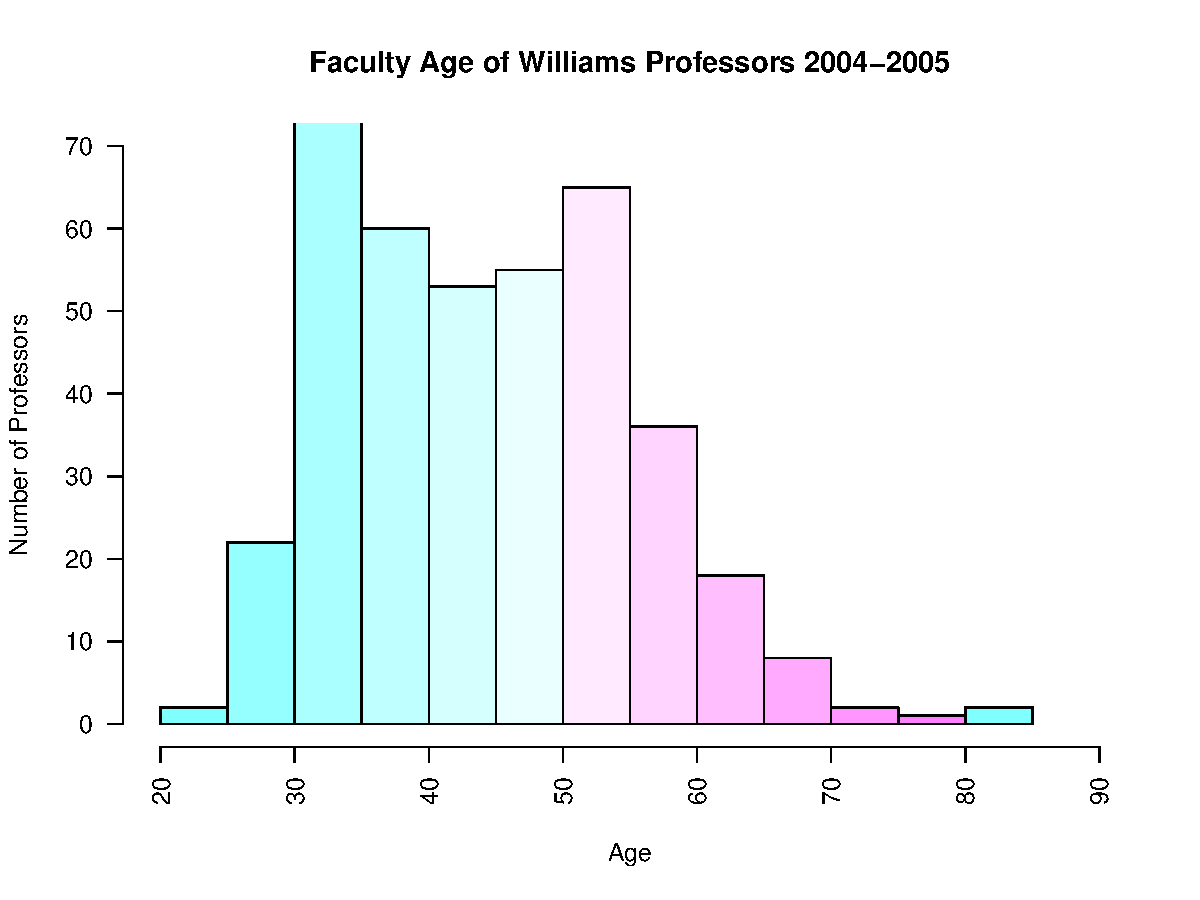
\includegraphics[width=\maxwidth]{figure/unnamed-chunk-9-1} 

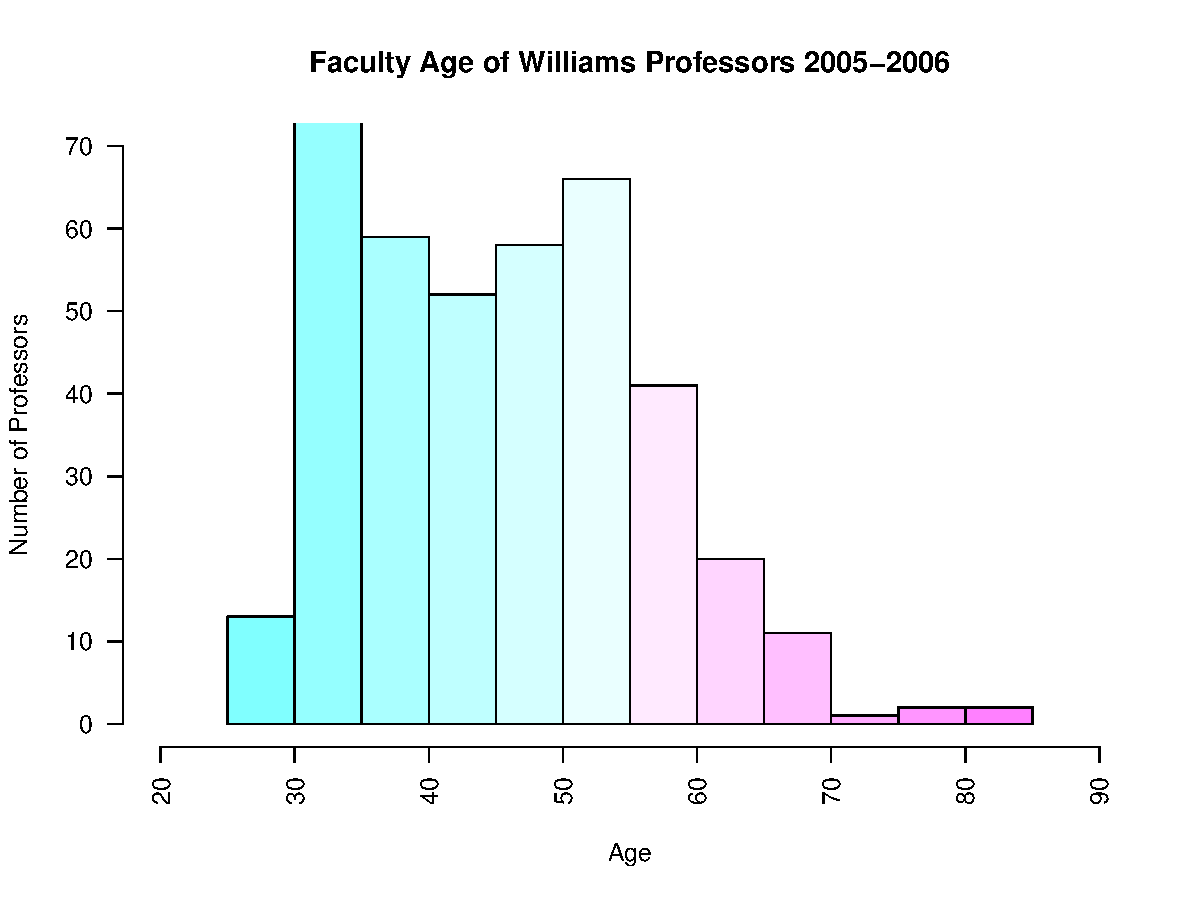
\includegraphics[width=\maxwidth]{figure/unnamed-chunk-9-2} 

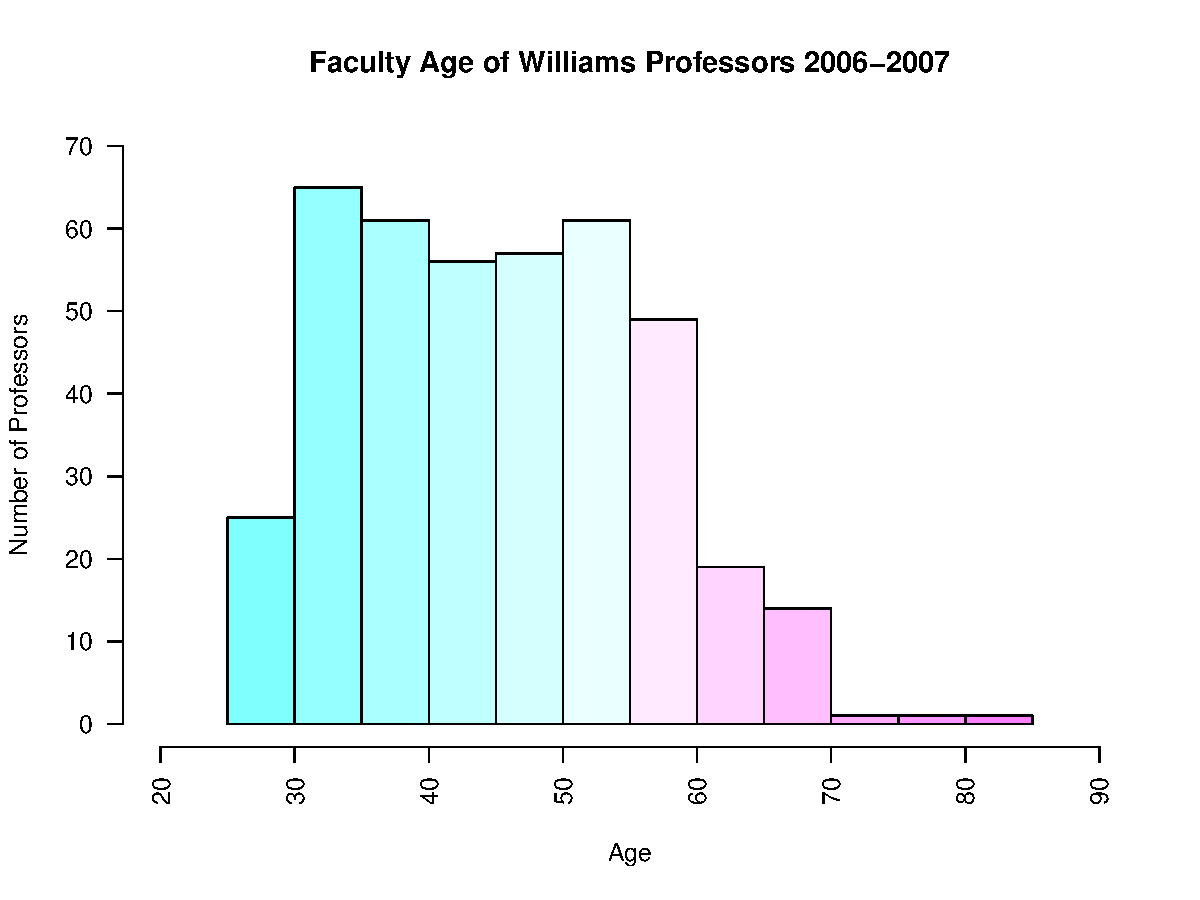
\includegraphics[width=\maxwidth]{figure/unnamed-chunk-9-3} 

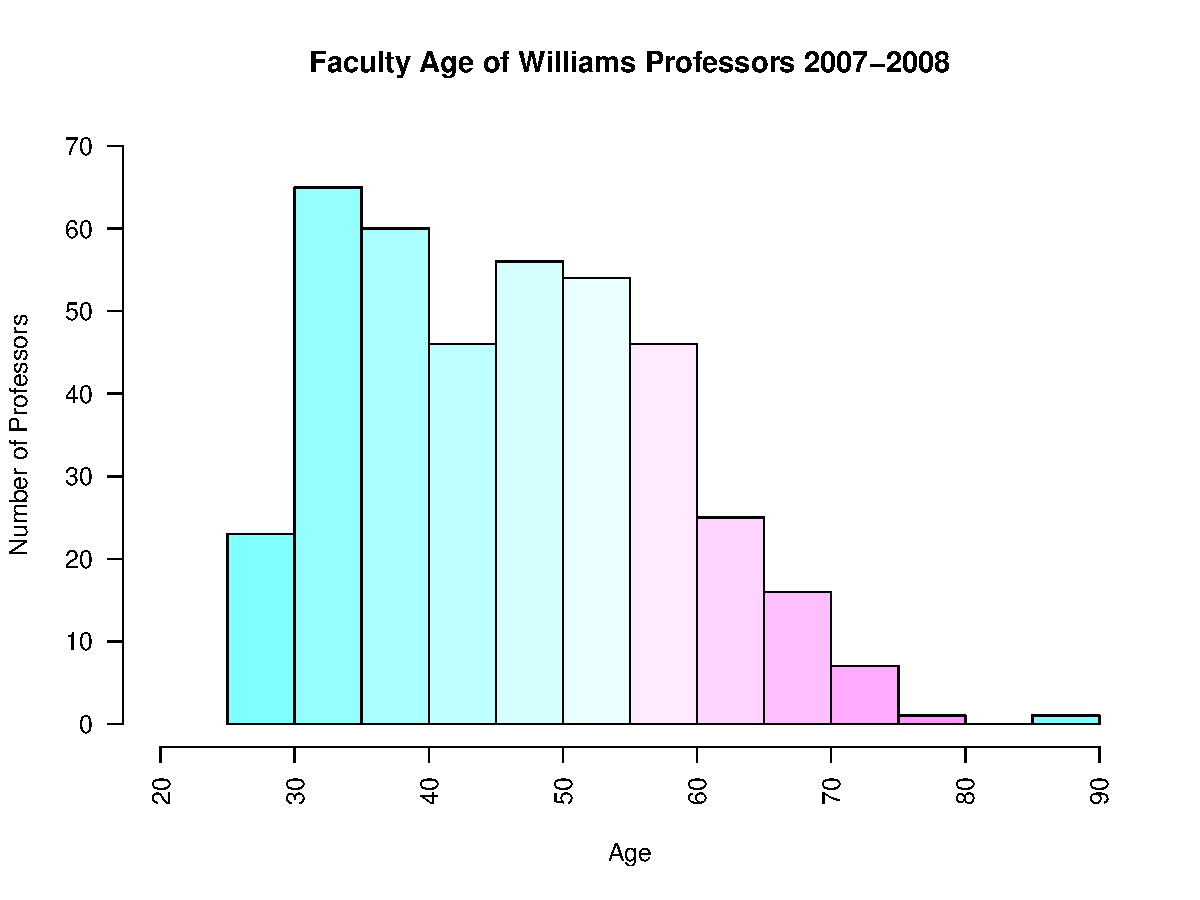
\includegraphics[width=\maxwidth]{figure/unnamed-chunk-9-4} 

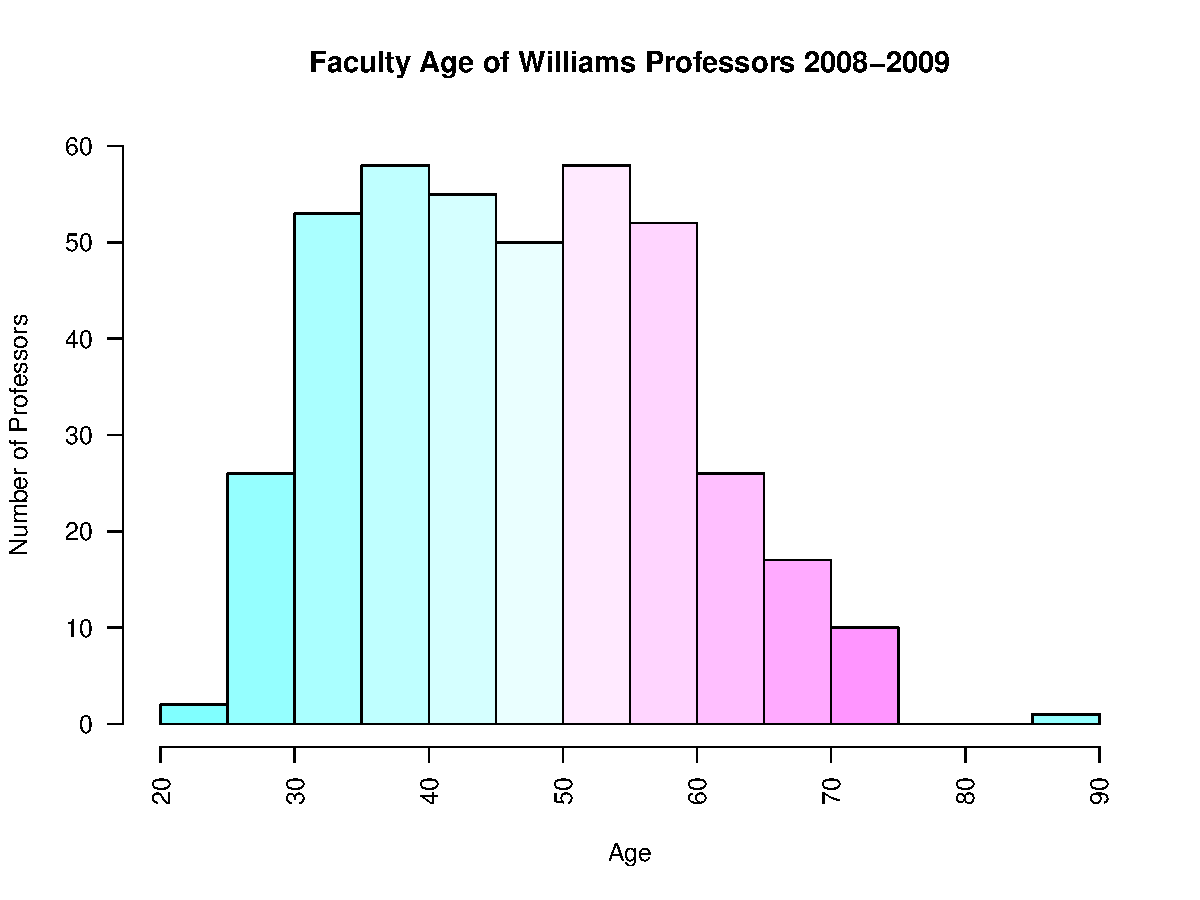
\includegraphics[width=\maxwidth]{figure/unnamed-chunk-9-5} 

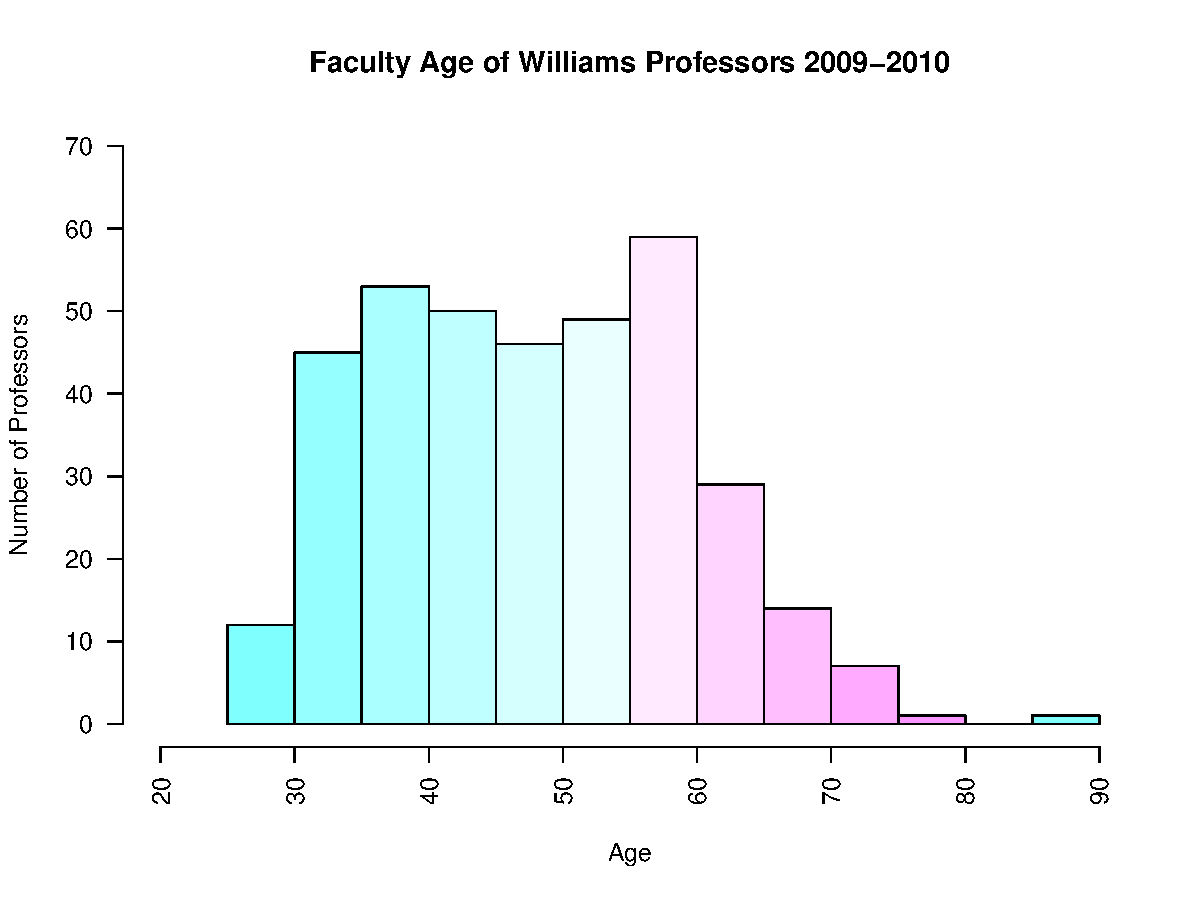
\includegraphics[width=\maxwidth]{figure/unnamed-chunk-9-6} 

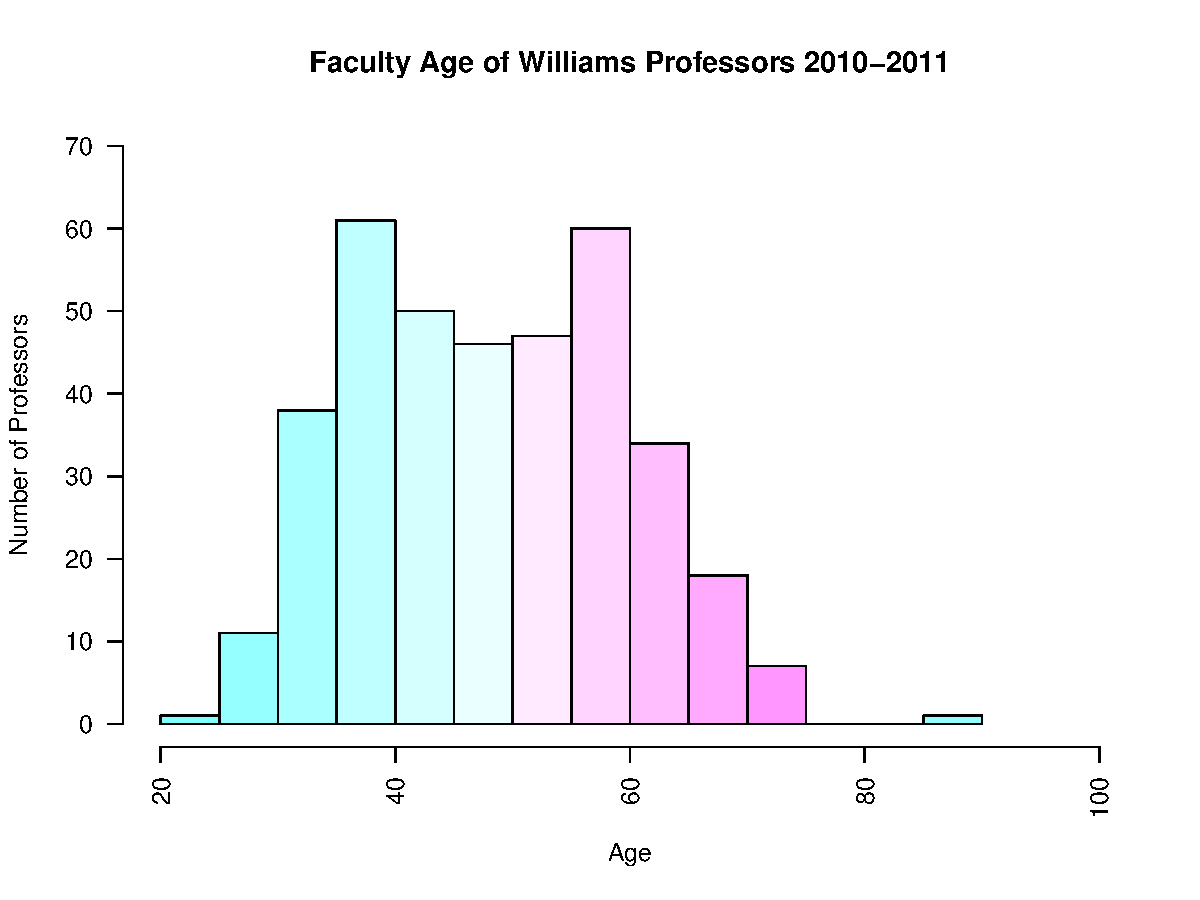
\includegraphics[width=\maxwidth]{figure/unnamed-chunk-9-7} 

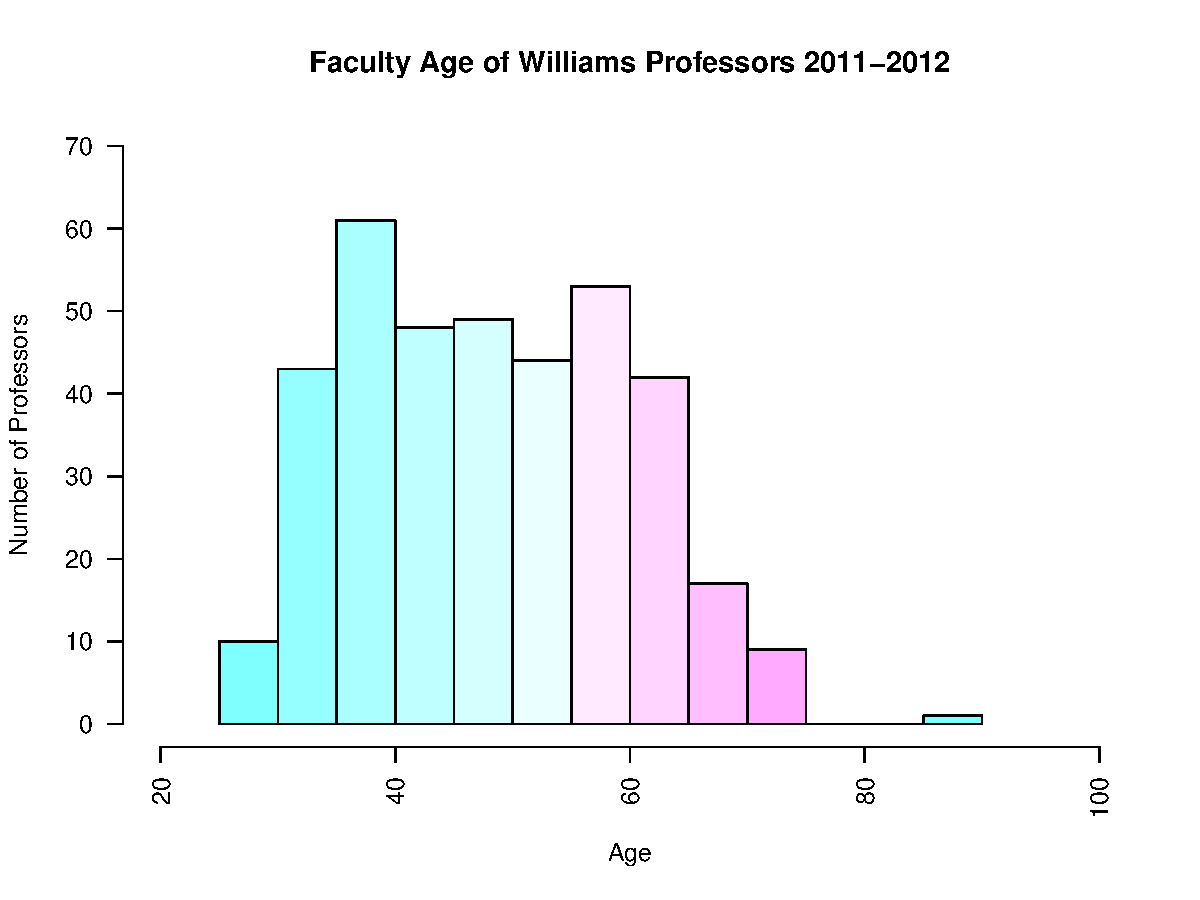
\includegraphics[width=\maxwidth]{figure/unnamed-chunk-9-8} 

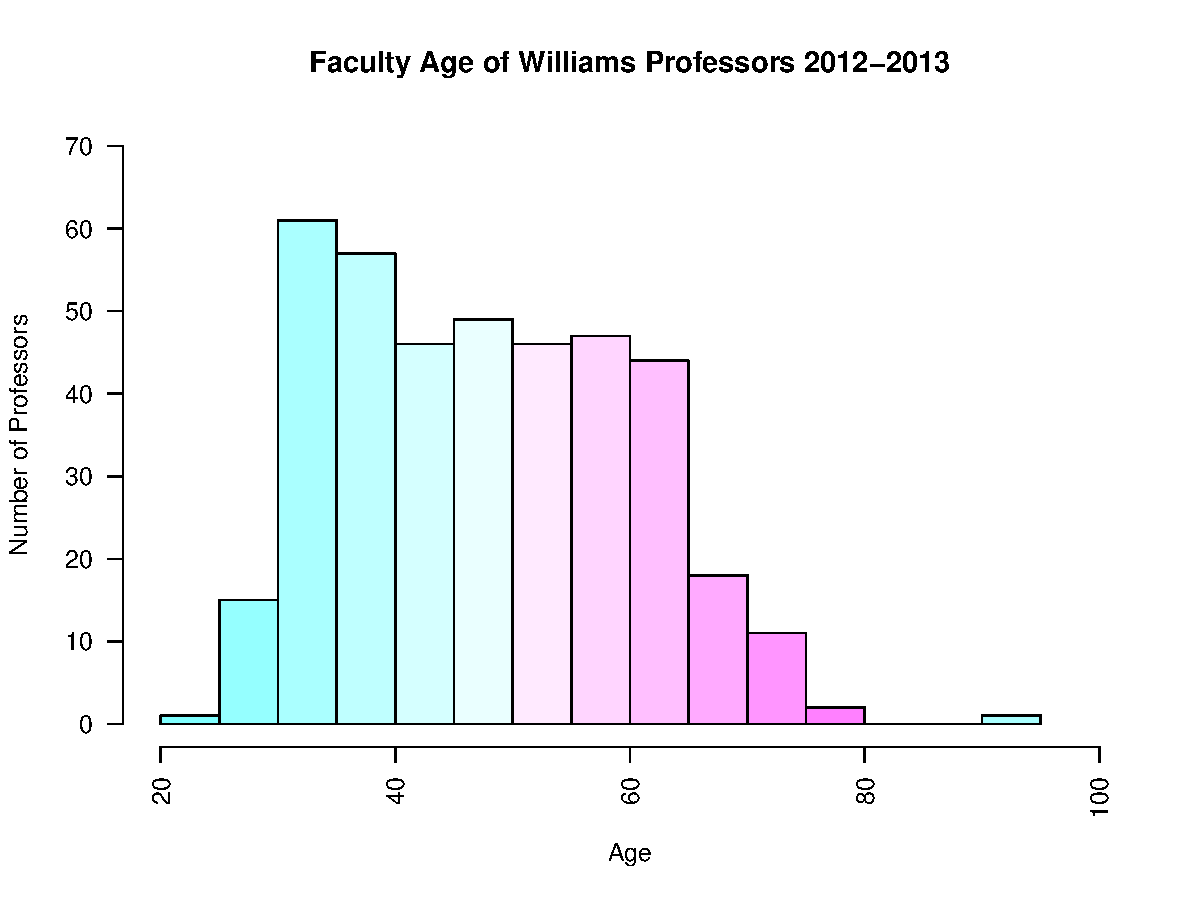
\includegraphics[width=\maxwidth]{figure/unnamed-chunk-9-9} 

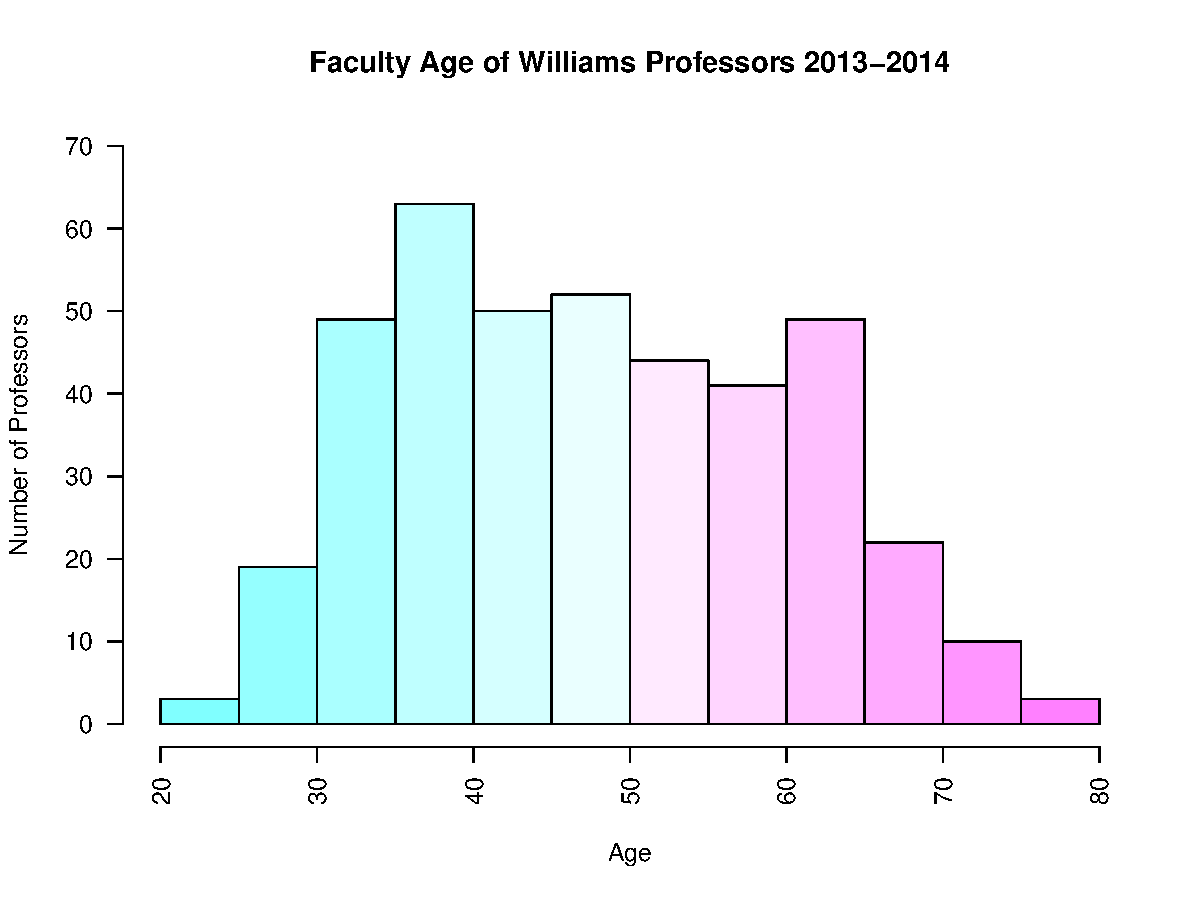
\includegraphics[width=\maxwidth]{figure/unnamed-chunk-9-10} 

\end{knitrout}

\bigskip
We see between the 2004-2005 and 2007-2008 academic years the age distribution is right-skewed, with the ages being primarily concentrated between 30 and 60. Between the 2008-2009 and 2012-2013 academic year display implies a fairly normal and symmetric age distribution of the faculty, with one outlier in the 85-90 age range. The ages continued to be primarily concentrated between 30 and 60, or 30 and 65. The 2012-2013 distribution is more right skewed than the other graphs and the outlier (Henry J. Bruton) is not apparent in the 2013-2014 display.

\bigskip
A key question in our analysis of the Williams College faculty for the past 10 years is the average age distribution by department and how it has changed over time. By examining barplot over the last 10 years it is interesting to observe the trends in the faculty member ages and how they are connected to departments.


\begin{knitrout}
\definecolor{shadecolor}{rgb}{0.969, 0.969, 0.969}\color{fgcolor}
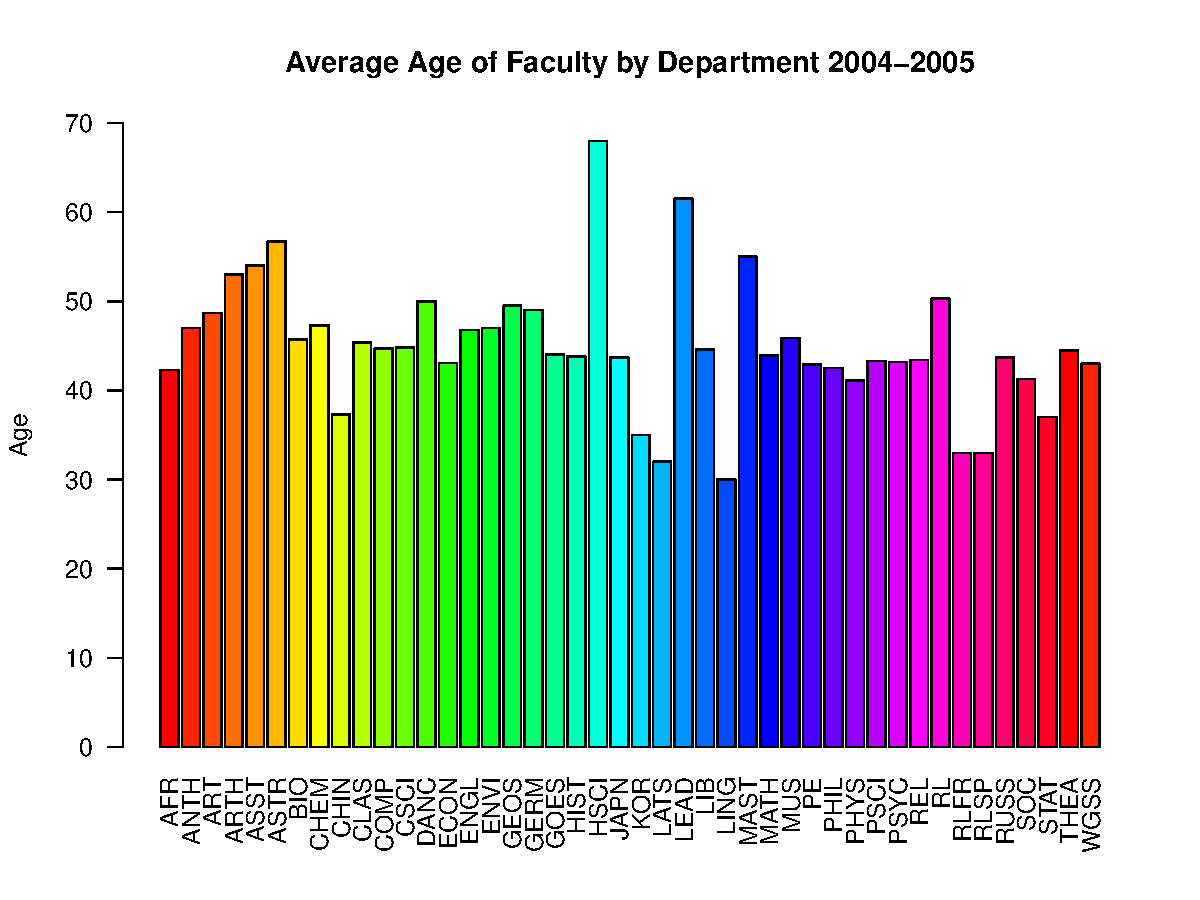
\includegraphics[width=\maxwidth]{figure/unnamed-chunk-10-1} 
\begin{kframe}\begin{verbatim}
## [1] "Average Age by Department 2004-2005:"
##  AFR ANTH  ART ARTH ASST ASTR  BIO CHEM CHIN CLAS COMP CSCI 
## 42.3 47.0 48.7 53.0 54.0 56.7 45.7 47.3 37.3 45.4 44.7 44.8 
## DANC ECON ENGL ENVI GEOS GERM GOES HIST HSCI JAPN  KOR LATS 
## 50.0 43.1 46.8 47.0 49.5 49.0 44.0 43.8 68.0 43.7 35.0 32.0 
## LEAD  LIB LING MAST MATH  MUS   PE PHIL PHYS PSCI PSYC  REL 
## 61.5 44.6 30.0 55.0 43.9 45.9 42.9 42.5 41.1 43.3 43.2 43.4 
##   RL RLFR RLSP RUSS  SOC STAT THEA WGSS 
## 50.3 33.0 33.0 43.7 41.3 37.0 44.5 43.0
\end{verbatim}
\end{kframe}
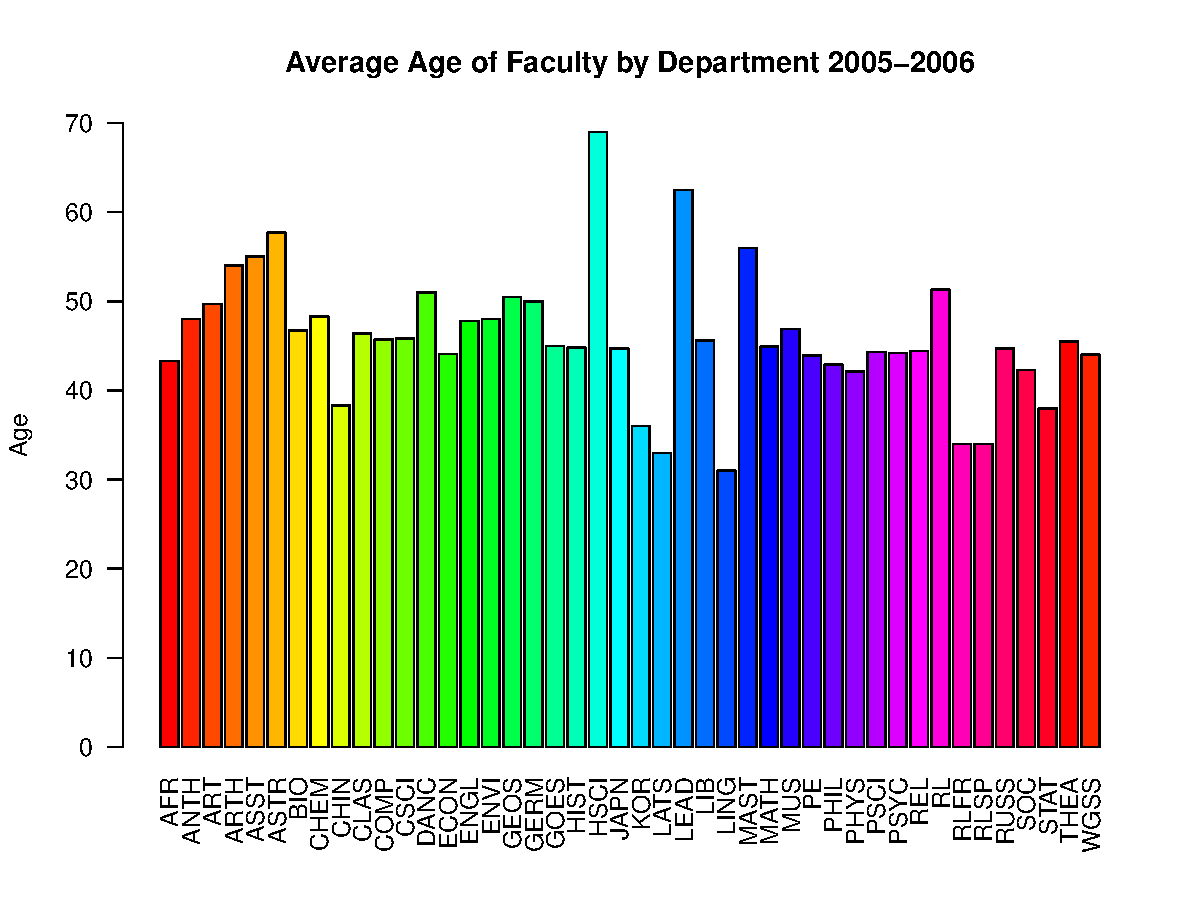
\includegraphics[width=\maxwidth]{figure/unnamed-chunk-10-2} 
\begin{kframe}\begin{verbatim}
## [1] "Average Age by Department 2005-2006:"
##  AFR ANTH  ART ARTH ASST ASTR  BIO CHEM CHIN CLAS COMP CSCI 
## 43.3 48.0 49.7 54.0 55.0 57.7 46.7 48.3 38.3 46.4 45.7 45.8 
## DANC ECON ENGL ENVI GEOS GERM GOES HIST HSCI JAPN  KOR LATS 
## 51.0 44.1 47.8 48.0 50.5 50.0 45.0 44.8 69.0 44.7 36.0 33.0 
## LEAD  LIB LING MAST MATH  MUS   PE PHIL PHYS PSCI PSYC  REL 
## 62.5 45.6 31.0 56.0 44.9 46.9 43.9 42.9 42.1 44.3 44.2 44.4 
##   RL RLFR RLSP RUSS  SOC STAT THEA WGSS 
## 51.3 34.0 34.0 44.7 42.3 38.0 45.5 44.0
\end{verbatim}
\end{kframe}
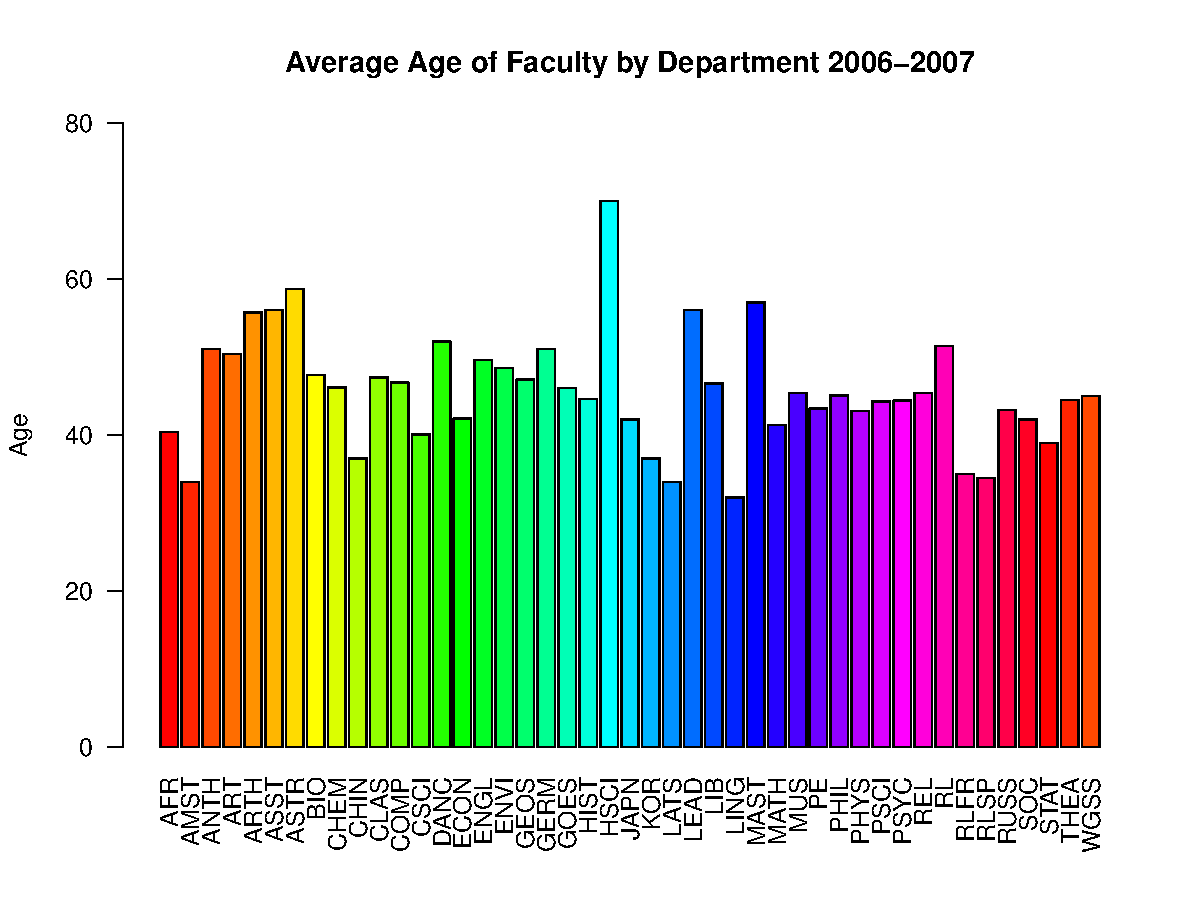
\includegraphics[width=\maxwidth]{figure/unnamed-chunk-10-3} 
\begin{kframe}\begin{verbatim}
## [1] "Average Age by Department 2006-2007:"
##  AFR AMST ANTH  ART ARTH ASST ASTR  BIO CHEM CHIN CLAS COMP 
## 40.4 34.0 51.0 50.4 55.7 56.0 58.7 47.7 46.1 37.0 47.4 46.7 
## CSCI DANC ECON ENGL ENVI GEOS GERM GOES HIST HSCI JAPN  KOR 
## 40.1 52.0 42.1 49.6 48.6 47.1 51.0 46.0 44.6 70.0 42.0 37.0 
## LATS LEAD  LIB LING MAST MATH  MUS   PE PHIL PHYS PSCI PSYC 
## 34.0 56.0 46.6 32.0 57.0 41.3 45.4 43.4 45.1 43.1 44.3 44.4 
##  REL   RL RLFR RLSP RUSS  SOC STAT THEA WGSS 
## 45.4 51.4 35.0 34.5 43.2 42.0 39.0 44.5 45.0
\end{verbatim}
\end{kframe}
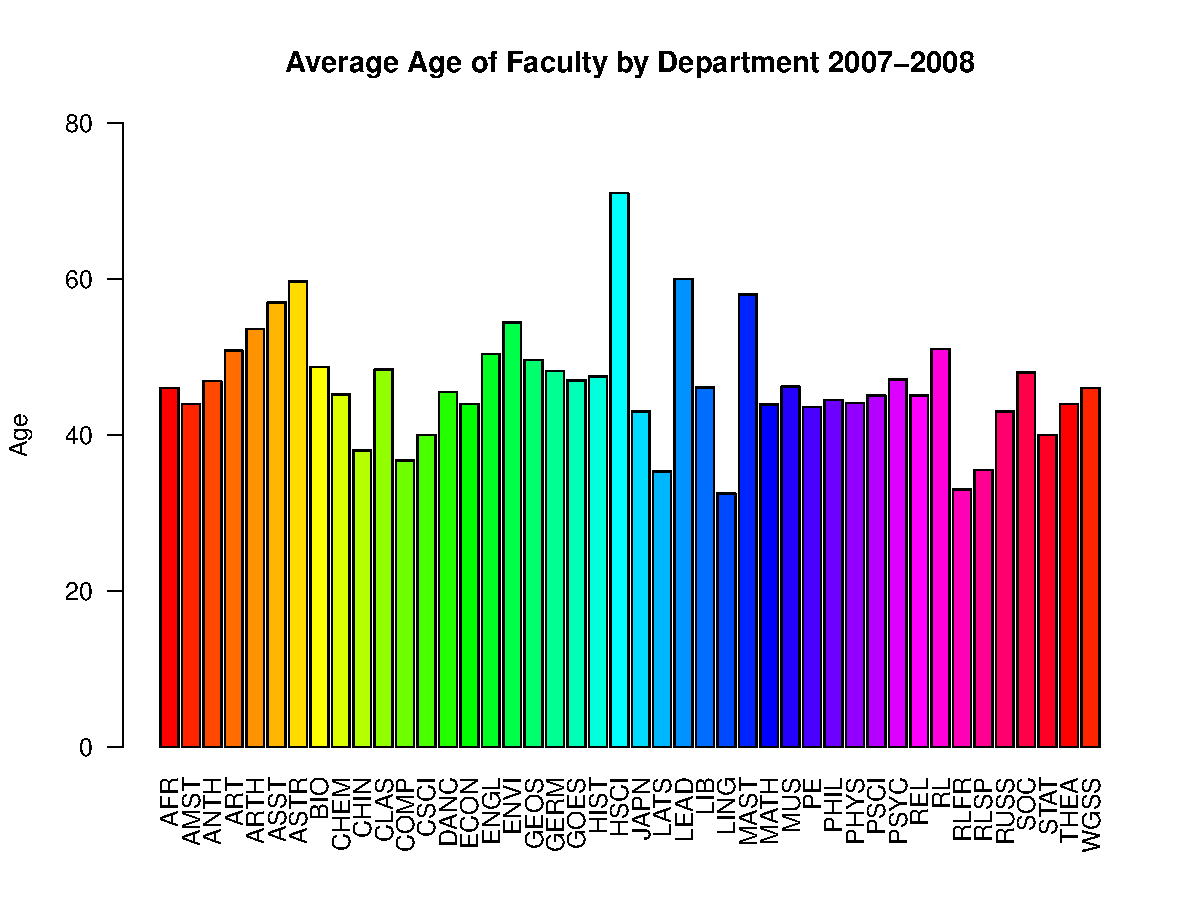
\includegraphics[width=\maxwidth]{figure/unnamed-chunk-10-4} 
\begin{kframe}\begin{verbatim}
## [1] "Average Age by Department 2007-2008:"
##  AFR AMST ANTH  ART ARTH ASST ASTR  BIO CHEM CHIN CLAS COMP 
## 46.0 44.0 46.9 50.8 53.6 57.0 59.7 48.7 45.2 38.0 48.4 36.7 
## CSCI DANC ECON ENGL ENVI GEOS GERM GOES HIST HSCI JAPN LATS 
## 40.0 45.5 44.0 50.4 54.4 49.6 48.2 47.0 47.5 71.0 43.0 35.3 
## LEAD  LIB LING MAST MATH  MUS   PE PHIL PHYS PSCI PSYC  REL 
## 60.0 46.1 32.5 58.0 43.9 46.2 43.6 44.5 44.1 45.1 47.1 45.1 
##   RL RLFR RLSP RUSS  SOC STAT THEA WGSS 
## 51.0 33.0 35.5 43.0 48.0 40.0 44.0 46.0
\end{verbatim}
\end{kframe}
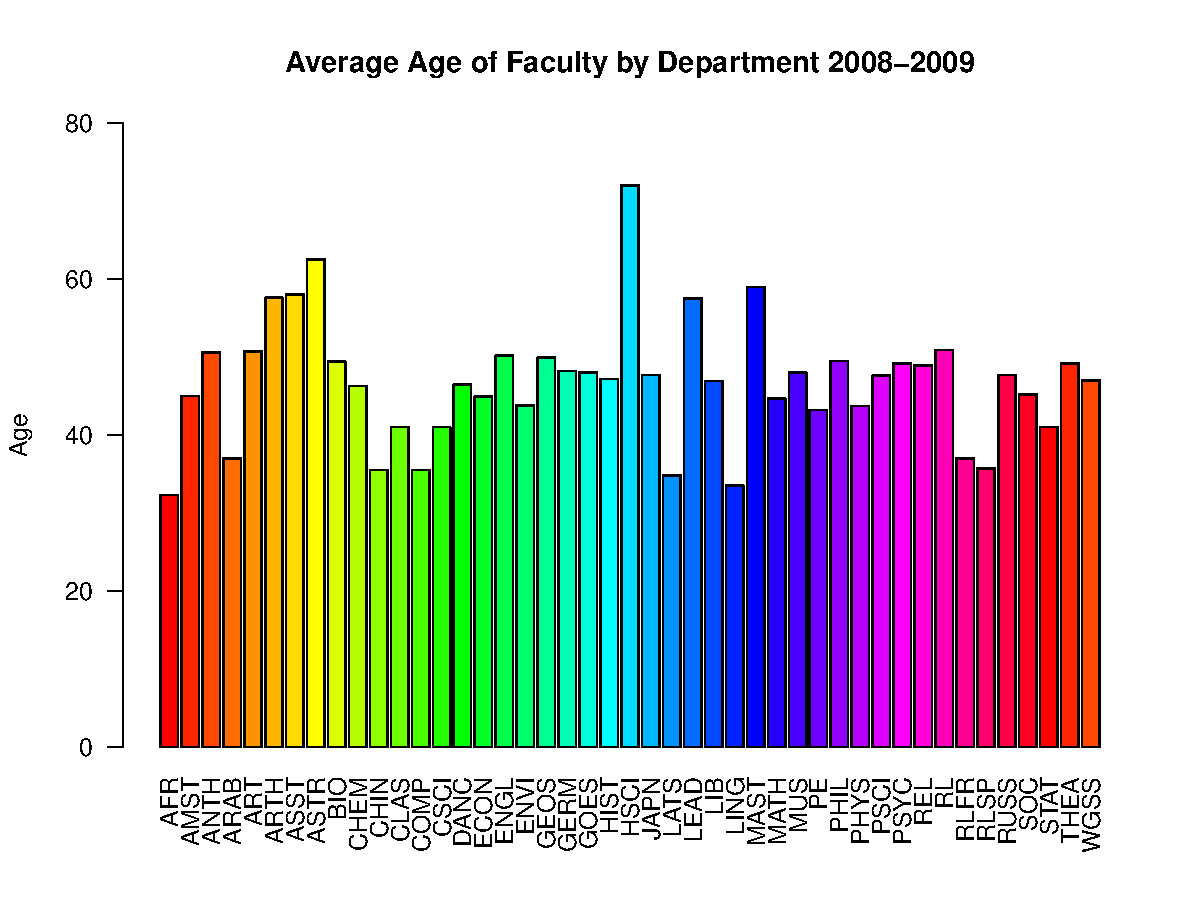
\includegraphics[width=\maxwidth]{figure/unnamed-chunk-10-5} 
\begin{kframe}\begin{verbatim}
## [1] "Average Age by Department 2008-2009:"
##  AFR AMST ANTH ARAB  ART ARTH ASST ASTR  BIO CHEM CHIN CLAS 
## 32.3 45.0 50.6 37.0 50.7 57.6 58.0 62.5 49.4 46.3 35.5 41.0 
## COMP CSCI DANC ECON ENGL ENVI GEOS GERM GOES HIST HSCI JAPN 
## 35.5 41.0 46.5 44.9 50.2 43.8 49.9 48.2 48.0 47.2 72.0 47.7 
## LATS LEAD  LIB LING MAST MATH  MUS   PE PHIL PHYS PSCI PSYC 
## 34.8 57.5 46.9 33.5 59.0 44.7 48.0 43.2 49.5 43.7 47.6 49.2 
##  REL   RL RLFR RLSP RUSS  SOC STAT THEA WGSS 
## 48.9 50.9 37.0 35.7 47.7 45.2 41.0 49.2 47.0
\end{verbatim}
\end{kframe}
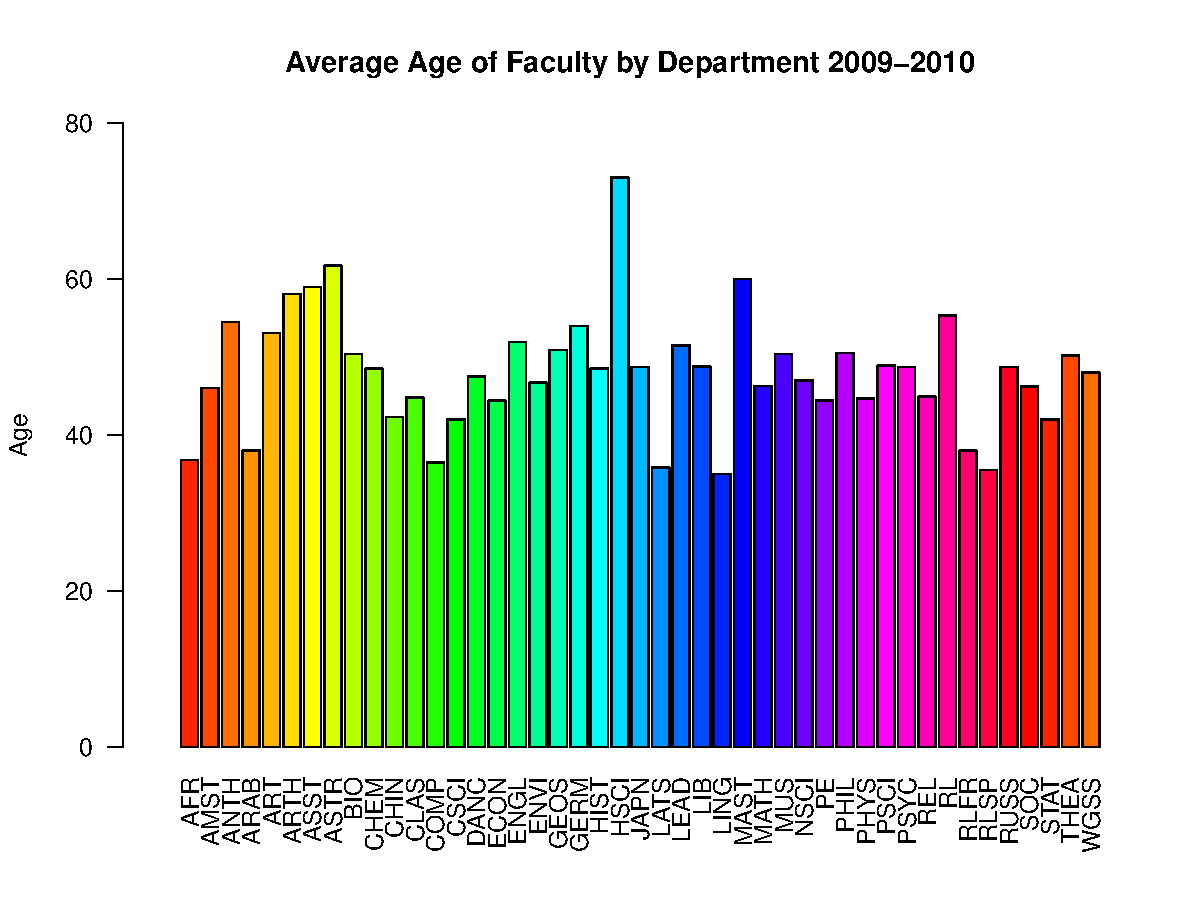
\includegraphics[width=\maxwidth]{figure/unnamed-chunk-10-6} 
\begin{kframe}\begin{verbatim}
## [1] "Average Age by Department 2009-2010:"
##       AFR AMST ANTH ARAB  ART ARTH ASST ASTR  BIO CHEM CHIN 
##   NA 36.8 46.0 54.5 38.0 53.1 58.1 59.0 61.7 50.4 48.5 42.3 
## CLAS COMP CSCI DANC ECON ENGL ENVI GEOS GERM HIST HSCI JAPN 
## 44.8 36.5 42.0 47.5 44.4 51.9 46.7 50.9 54.0 48.5 73.0 48.7 
## LATS LEAD  LIB LING MAST MATH  MUS NSCI   PE PHIL PHYS PSCI 
## 35.8 51.5 48.8 35.0 60.0 46.3 50.4 47.0 44.4 50.5 44.7 48.9 
## PSYC  REL   RL RLFR RLSP RUSS  SOC STAT THEA WGSS 
## 48.7 44.9 55.3 38.0 35.5 48.7 46.2 42.0 50.2 48.0
\end{verbatim}
\end{kframe}
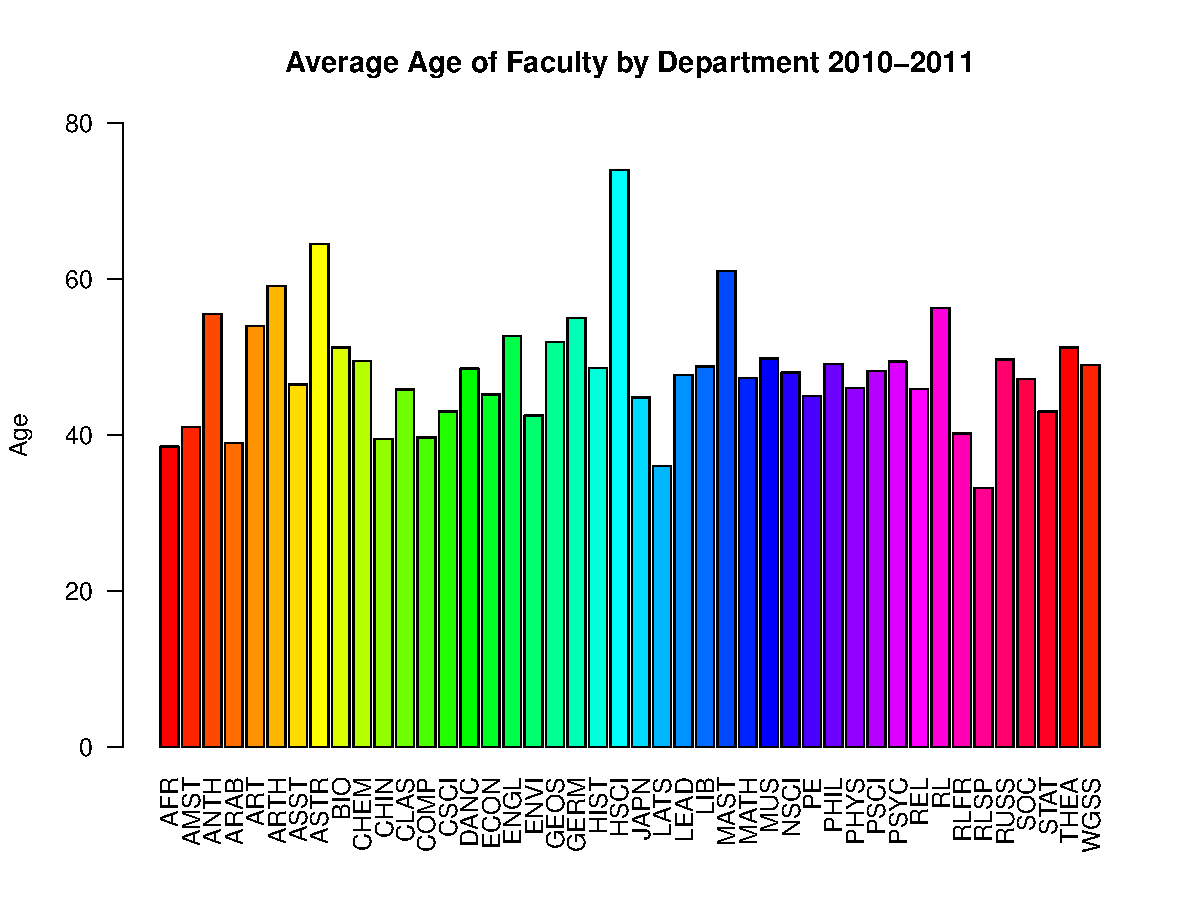
\includegraphics[width=\maxwidth]{figure/unnamed-chunk-10-7} 
\begin{kframe}\begin{verbatim}
## [1] "Average Age by Department 2010-2011:"
##  AFR AMST ANTH ARAB  ART ARTH ASST ASTR  BIO CHEM CHIN CLAS 
## 38.5 41.0 55.5 39.0 54.0 59.1 46.5 64.5 51.2 49.5 39.5 45.8 
## COMP CSCI DANC ECON ENGL ENVI GEOS GERM HIST HSCI JAPN LATS 
## 39.7 43.0 48.5 45.2 52.7 42.5 51.9 55.0 48.6 74.0 44.8 36.0 
## LEAD  LIB MAST MATH  MUS NSCI   PE PHIL PHYS PSCI PSYC  REL 
## 47.7 48.8 61.0 47.3 49.8 48.0 45.0 49.1 46.0 48.2 49.4 45.9 
##   RL RLFR RLSP RUSS  SOC STAT THEA WGSS 
## 56.3 40.2 33.2 49.7 47.2 43.0 51.2 49.0
\end{verbatim}
\end{kframe}
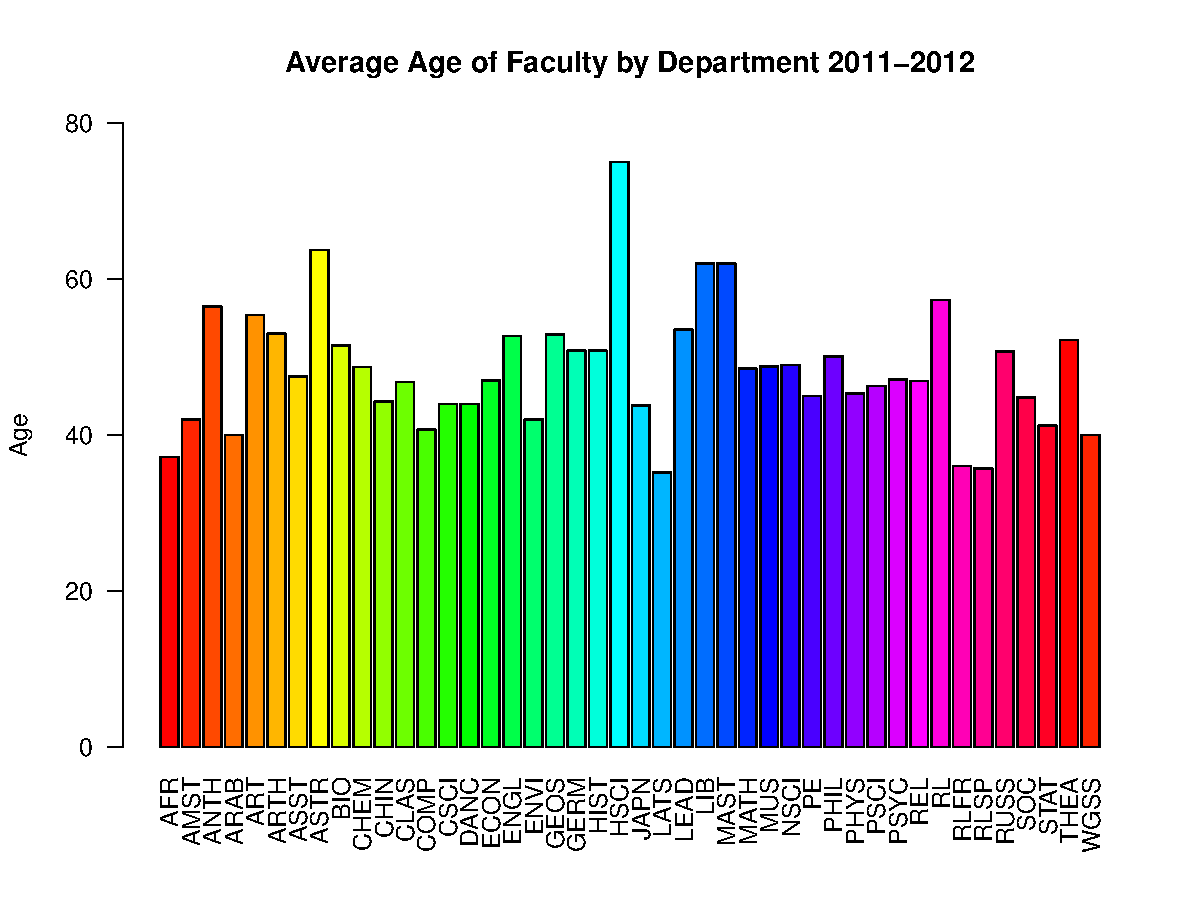
\includegraphics[width=\maxwidth]{figure/unnamed-chunk-10-8} 
\begin{kframe}\begin{verbatim}
## [1] "Average Age by Department 2011-2012:"
##  AFR AMST ANTH ARAB  ART ARTH ASST ASTR  BIO CHEM CHIN CLAS 
## 37.2 42.0 56.5 40.0 55.4 53.0 47.5 63.7 51.5 48.7 44.3 46.8 
## COMP CSCI DANC ECON ENGL ENVI GEOS GERM HIST HSCI JAPN LATS 
## 40.7 44.0 44.0 47.0 52.7 42.0 52.9 50.8 50.8 75.0 43.8 35.2 
## LEAD  LIB MAST MATH  MUS NSCI   PE PHIL PHYS PSCI PSYC  REL 
## 53.5 62.0 62.0 48.5 48.8 49.0 45.0 50.1 45.3 46.3 47.1 46.9 
##   RL RLFR RLSP RUSS  SOC STAT THEA WGSS 
## 57.3 36.0 35.7 50.7 44.8 41.2 52.2 40.0
\end{verbatim}
\end{kframe}
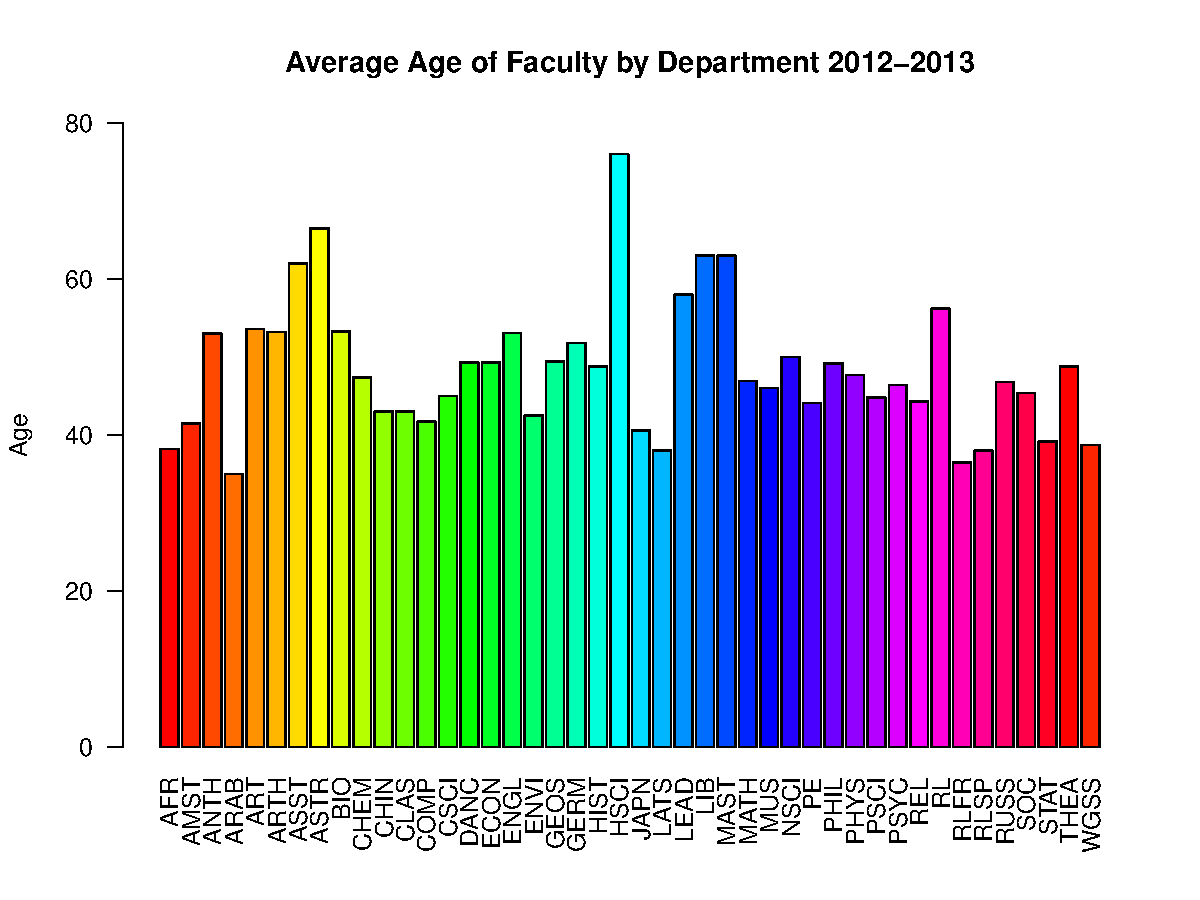
\includegraphics[width=\maxwidth]{figure/unnamed-chunk-10-9} 
\begin{kframe}\begin{verbatim}
## [1] "Average Age by Department 2012-2013:"
##  AFR AMST ANTH ARAB  ART ARTH ASST ASTR  BIO CHEM CHIN CLAS 
## 38.2 41.5 53.0 35.0 53.6 53.2 62.0 66.5 53.3 47.4 43.0 43.0 
## COMP CSCI DANC ECON ENGL ENVI GEOS GERM HIST HSCI JAPN LATS 
## 41.7 45.0 49.3 49.3 53.1 42.5 49.4 51.8 48.8 76.0 40.6 38.0 
## LEAD  LIB MAST MATH  MUS NSCI   PE PHIL PHYS PSCI PSYC  REL 
## 58.0 63.0 63.0 46.9 46.0 50.0 44.1 49.2 47.7 44.8 46.4 44.3 
##   RL RLFR RLSP RUSS  SOC STAT THEA WGSS 
## 56.2 36.5 38.0 46.8 45.4 39.2 48.8 38.7
\end{verbatim}
\end{kframe}
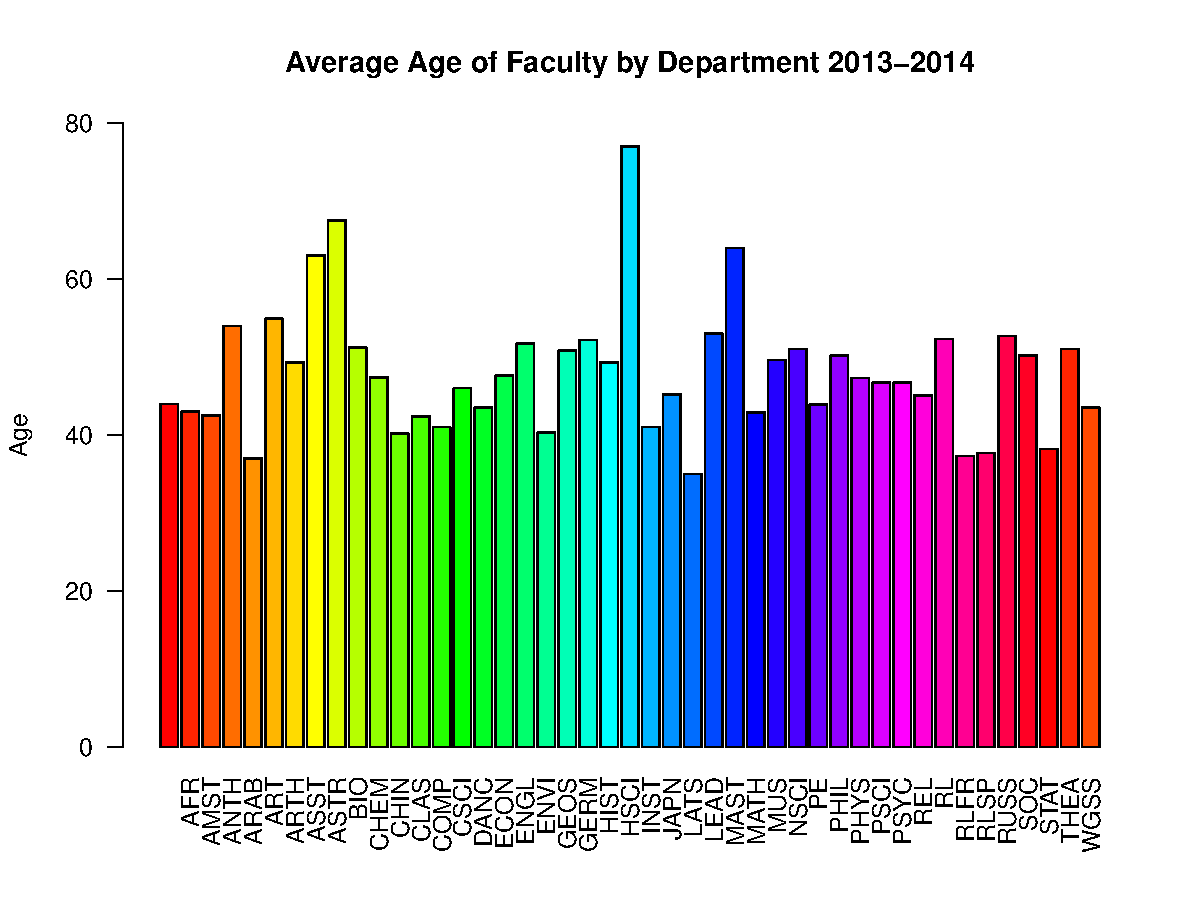
\includegraphics[width=\maxwidth]{figure/unnamed-chunk-10-10} 
\begin{kframe}\begin{verbatim}
## [1] "Average Age by Department 2013-2014:"
##       AFR AMST ANTH ARAB  ART ARTH ASST ASTR  BIO CHEM CHIN 
## 44.0 43.0 42.5 54.0 37.0 54.9 49.3 63.0 67.5 51.2 47.4 40.2 
## CLAS COMP CSCI DANC ECON ENGL ENVI GEOS GERM HIST HSCI INST 
## 42.4 41.0 46.0 43.5 47.6 51.7 40.3 50.8 52.2 49.3 77.0 41.0 
## JAPN LATS LEAD MAST MATH  MUS NSCI   PE PHIL PHYS PSCI PSYC 
## 45.2 35.0 53.0 64.0 42.9 49.6 51.0 43.9 50.2 47.3 46.7 46.7 
##  REL   RL RLFR RLSP RUSS  SOC STAT THEA WGSS 
## 45.1 52.3 37.3 37.7 52.7 50.2 38.2 51.0 43.5
\end{verbatim}
\end{kframe}
\end{knitrout}

\bigskip
It appears as though most of the department ages tend to be concentrated around 45 to 50, with a small number of departments being at the low and high ends. The Martime Studies, History of Science, Astronomy, Anthropology departments tended to be consistently on the high end, while the language departments like Arabic, Japanese, French, Spanish, Linguistics, Chinese, as well as Latino and Africana Studies tended to be at the low end.

\bigskip
Next, we analyze how the average age of the Williams College faculty for the past 10 years is different by gender. By examining barplots over the last 10 years it is easy to observe the difference between the average age of the male and female faculty.


\begin{knitrout}
\definecolor{shadecolor}{rgb}{0.969, 0.969, 0.969}\color{fgcolor}
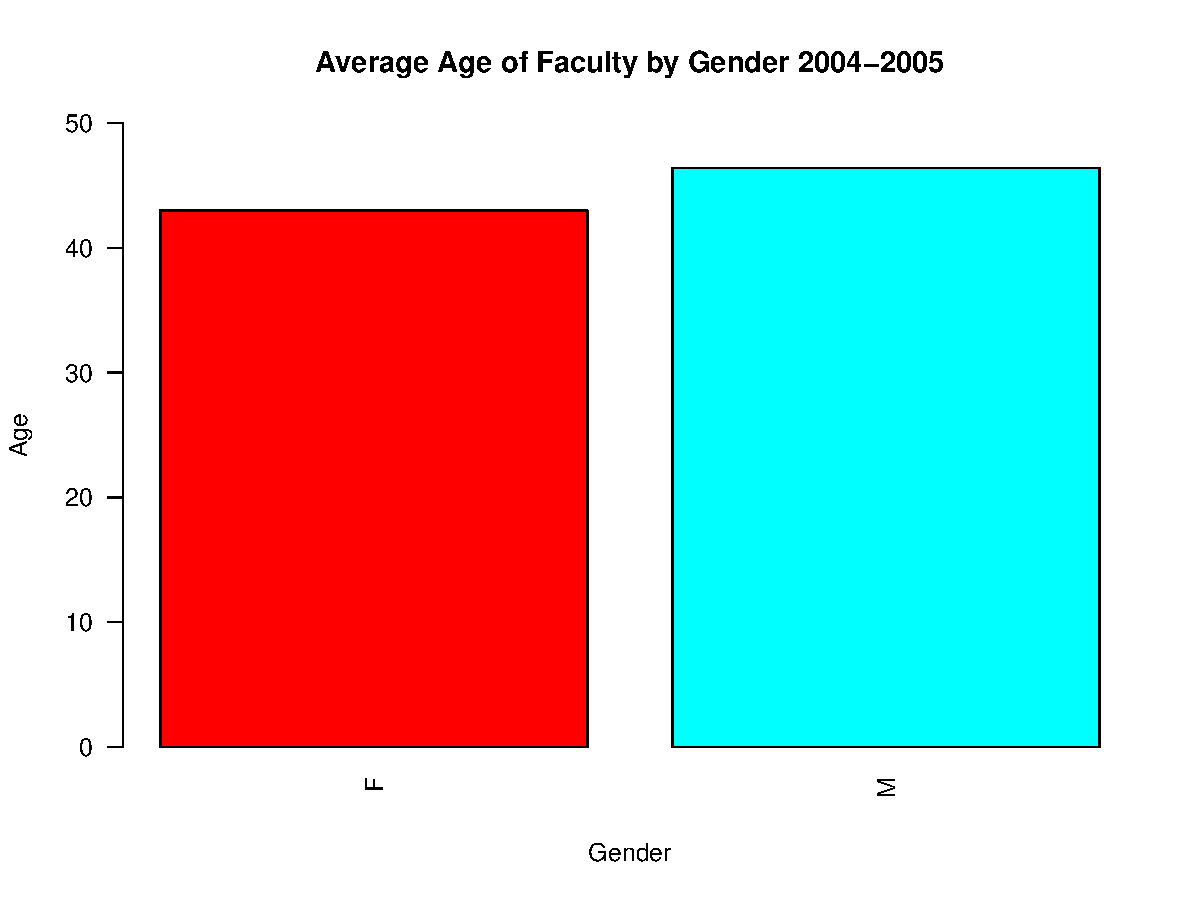
\includegraphics[width=\maxwidth]{figure/unnamed-chunk-11-1} 
\begin{kframe}\begin{verbatim}
## [1] "Average Age by Gender 2004-2005:"
##    F    M 
## 43.0 46.4
\end{verbatim}
\end{kframe}
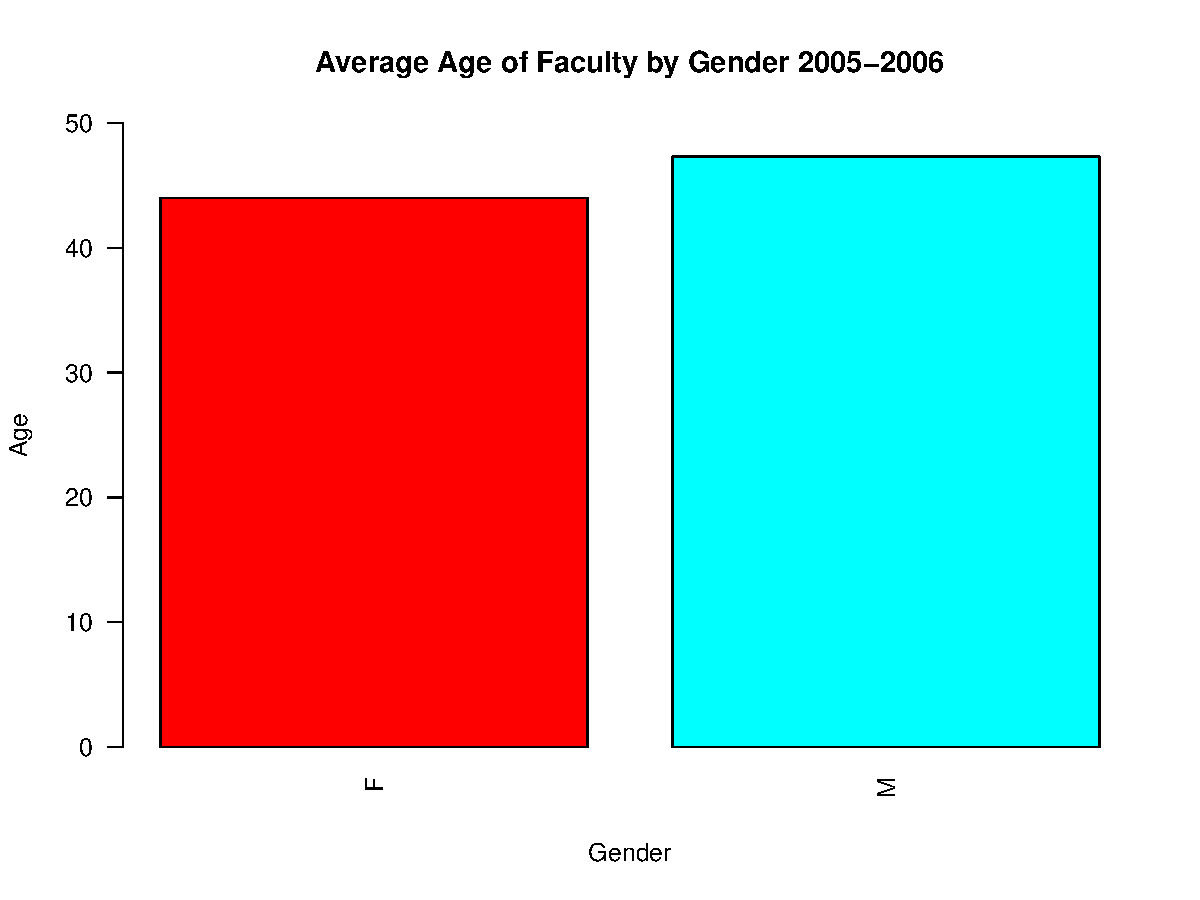
\includegraphics[width=\maxwidth]{figure/unnamed-chunk-11-2} 
\begin{kframe}\begin{verbatim}
## [1] "Average Age by Gender 2005-2006:"
##    F    M 
## 44.0 47.3
\end{verbatim}
\end{kframe}
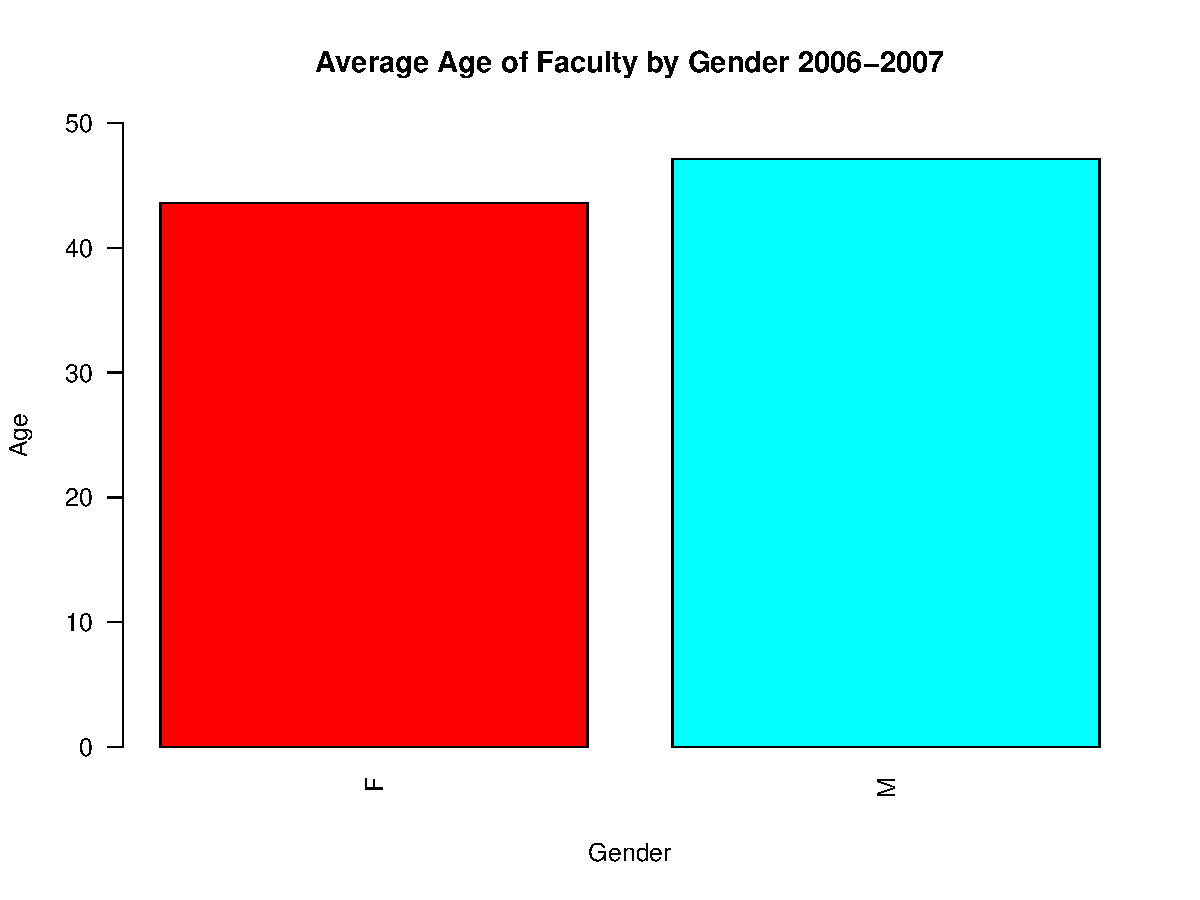
\includegraphics[width=\maxwidth]{figure/unnamed-chunk-11-3} 
\begin{kframe}\begin{verbatim}
## [1] "Average Age by Gender 2006-2007:"
##    F    M 
## 43.6 47.1
\end{verbatim}
\end{kframe}
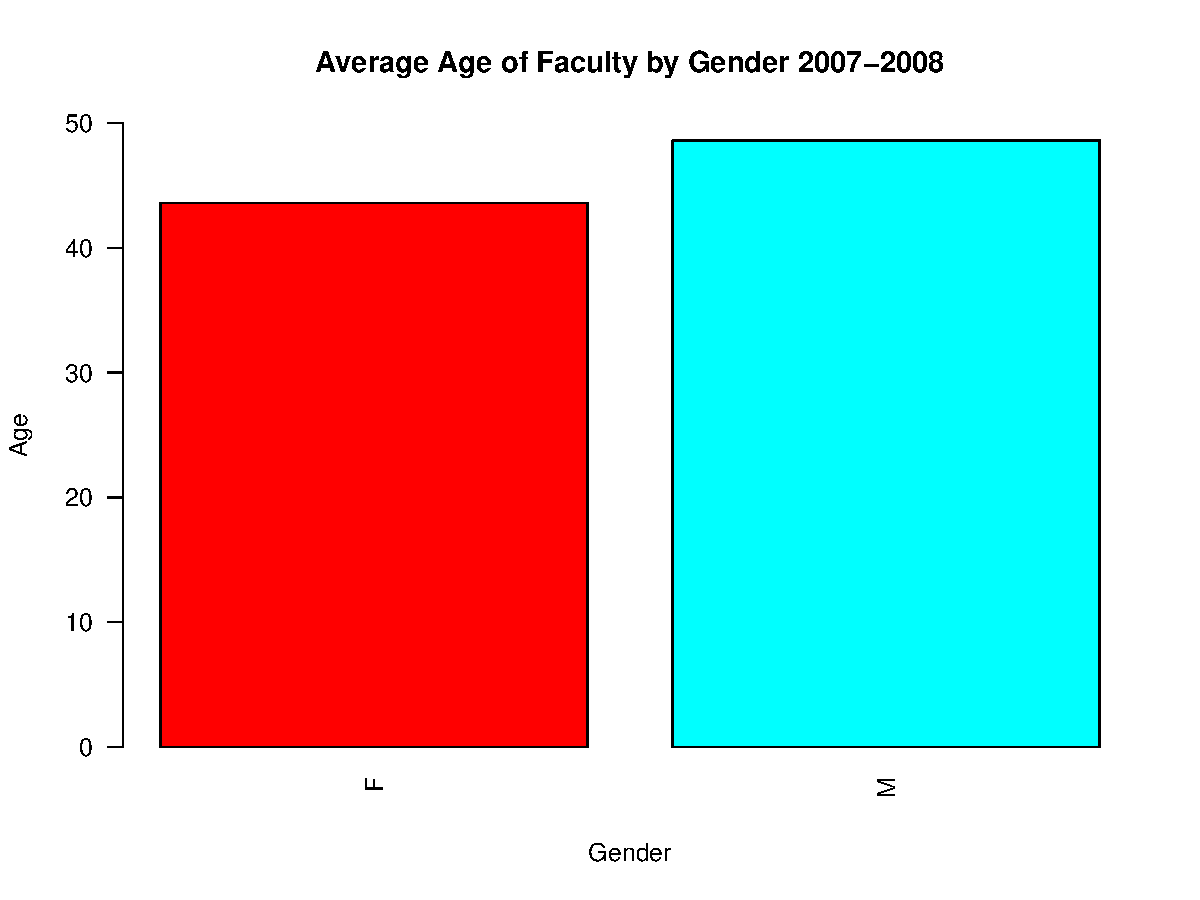
\includegraphics[width=\maxwidth]{figure/unnamed-chunk-11-4} 
\begin{kframe}\begin{verbatim}
## [1] "Average Age by Gender 2007-2008:"
##    F    M 
## 43.6 48.6
\end{verbatim}
\end{kframe}
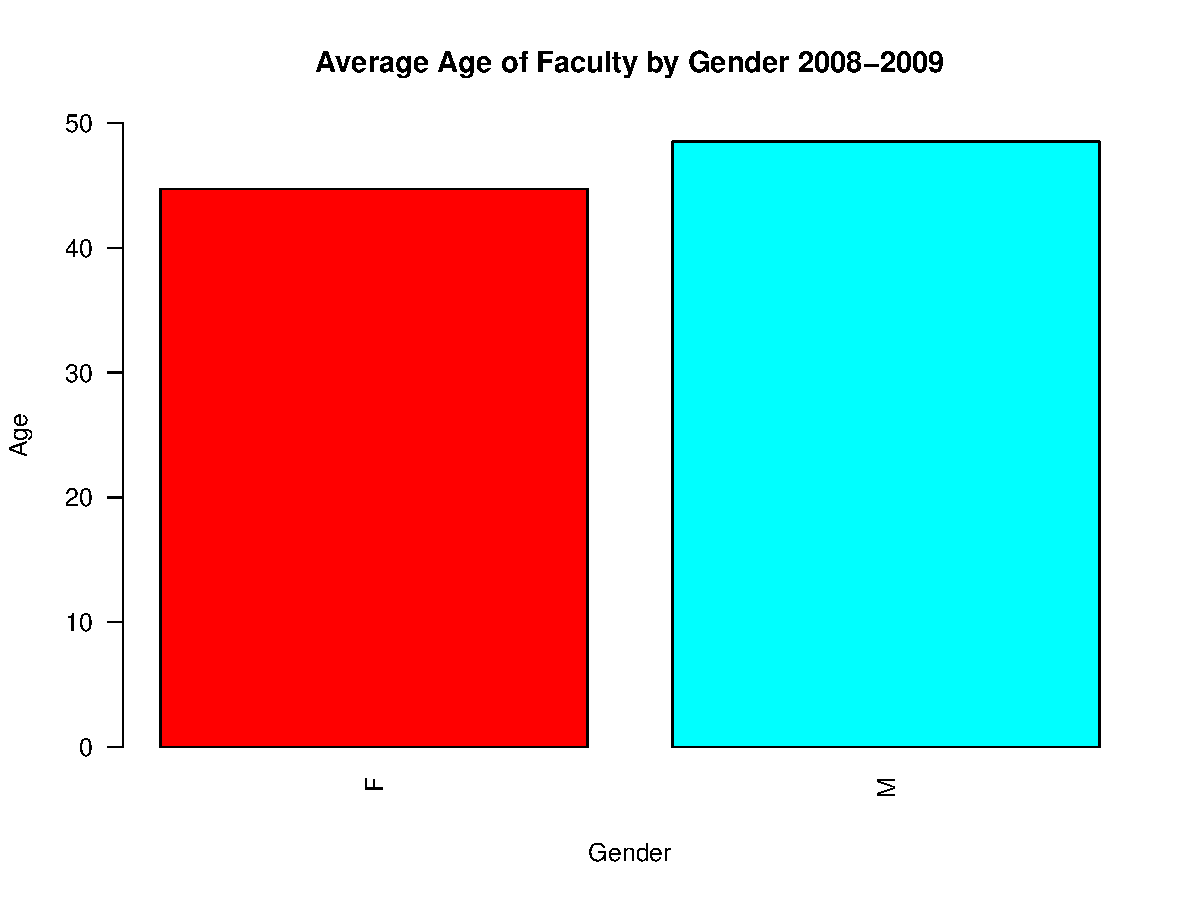
\includegraphics[width=\maxwidth]{figure/unnamed-chunk-11-5} 
\begin{kframe}\begin{verbatim}
## [1] "Average Age by Gender 2008-2009:"
##    F    M 
## 44.7 48.5
\end{verbatim}
\end{kframe}
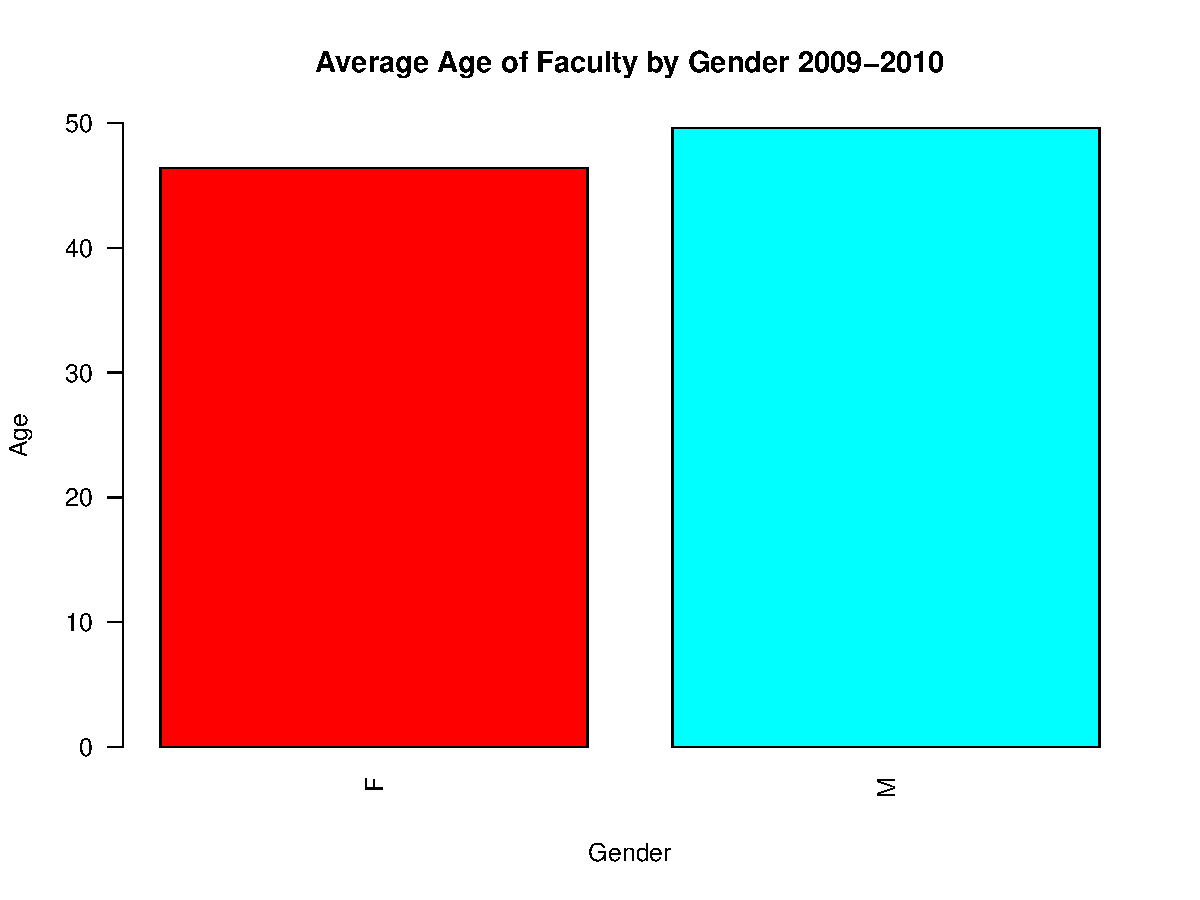
\includegraphics[width=\maxwidth]{figure/unnamed-chunk-11-6} 
\begin{kframe}\begin{verbatim}
## [1] "Average Age by Gender 2009-2010:"
##    F    M 
## 46.4 49.6
\end{verbatim}
\end{kframe}
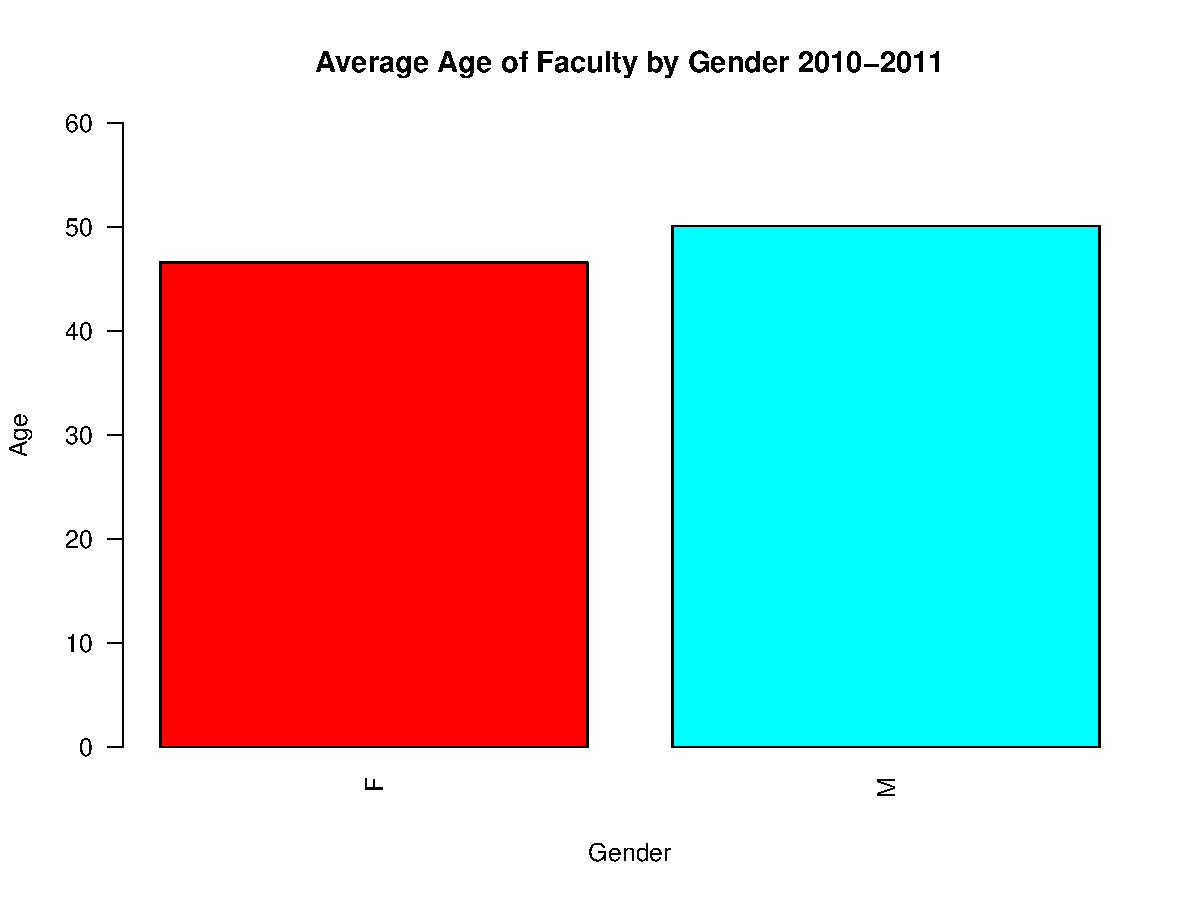
\includegraphics[width=\maxwidth]{figure/unnamed-chunk-11-7} 
\begin{kframe}\begin{verbatim}
## [1] "Average Age by Gender 2010-2011:"
##    F    M 
## 46.6 50.1
\end{verbatim}
\end{kframe}
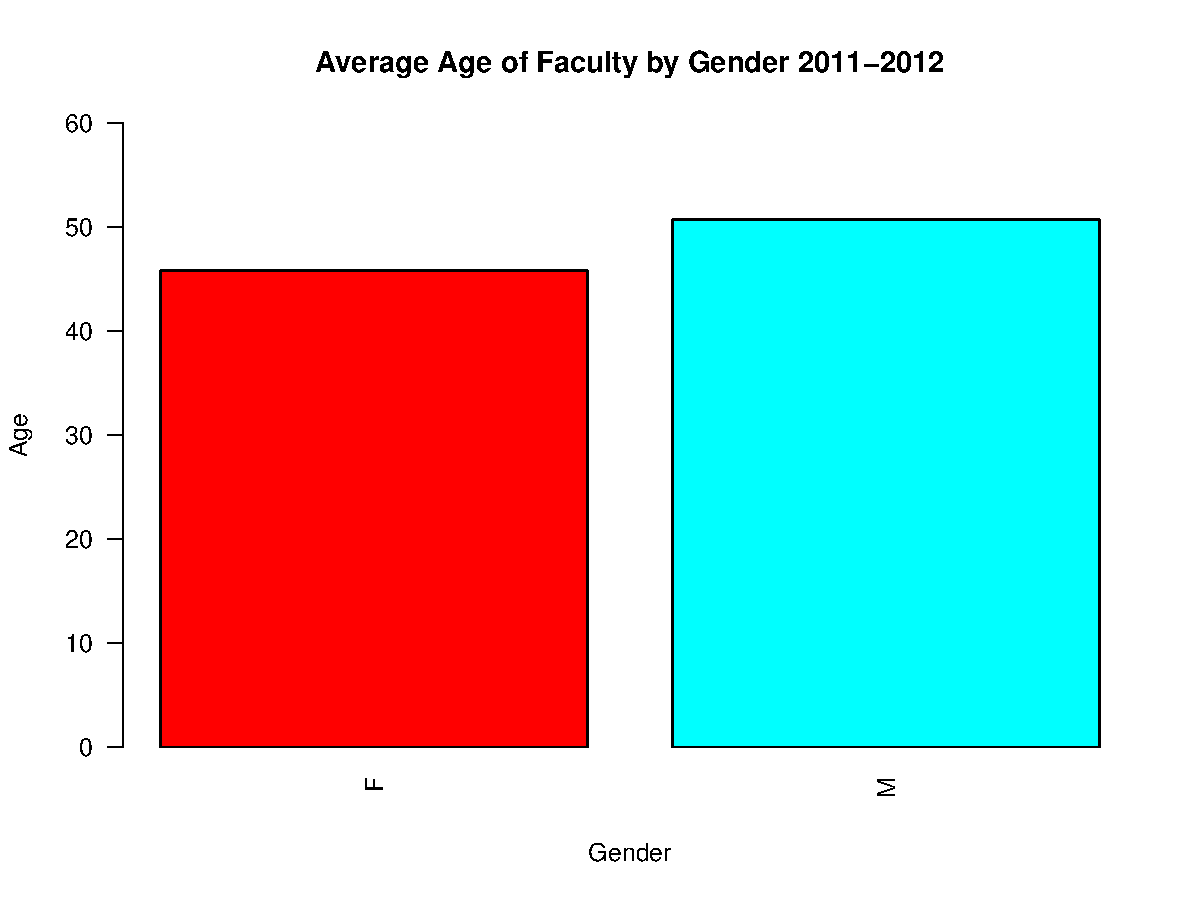
\includegraphics[width=\maxwidth]{figure/unnamed-chunk-11-8} 
\begin{kframe}\begin{verbatim}
## [1] "Average Age by Gender 2011-2012:"
##    F    M 
## 45.8 50.7
\end{verbatim}
\end{kframe}
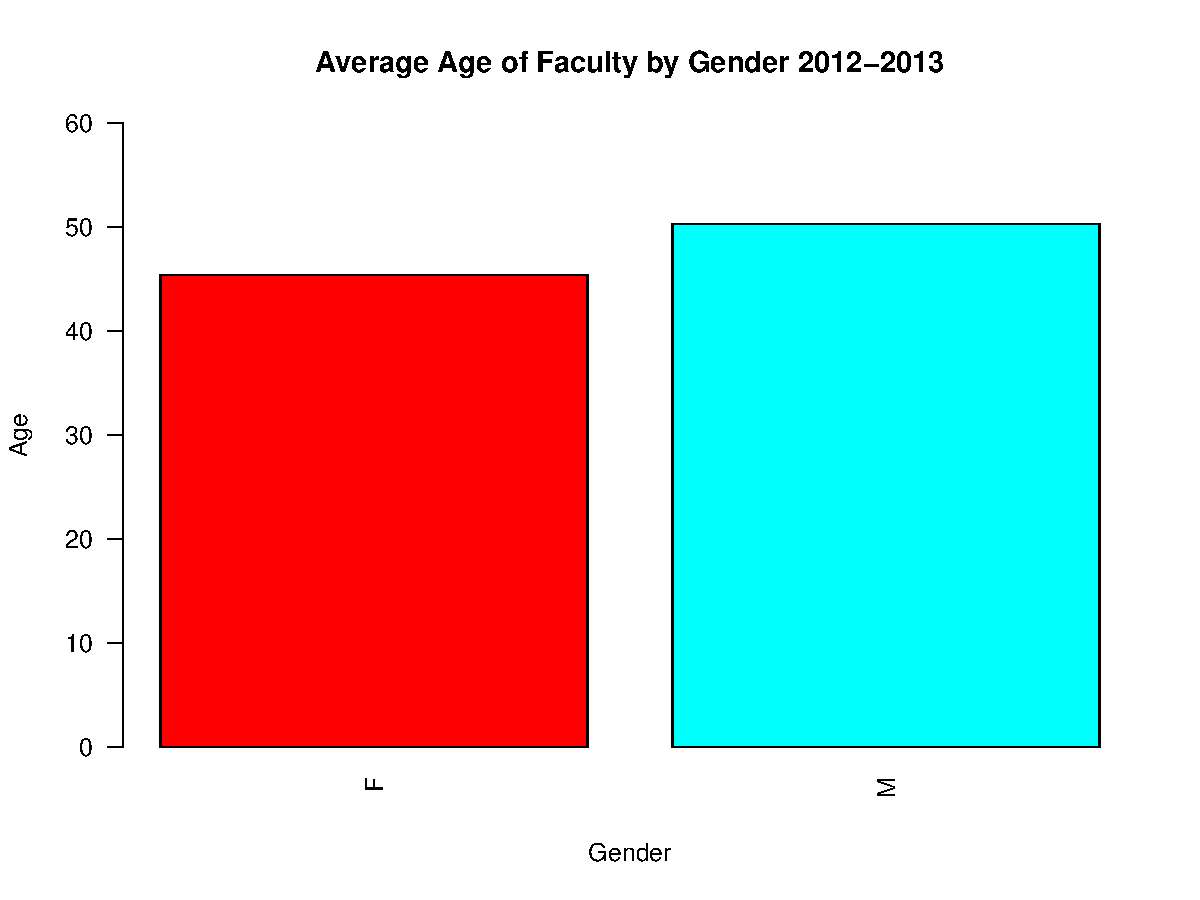
\includegraphics[width=\maxwidth]{figure/unnamed-chunk-11-9} 
\begin{kframe}\begin{verbatim}
## [1] "Average Age by Gender 2012-2013:"
##    F    M 
## 45.4 50.3
\end{verbatim}
\end{kframe}
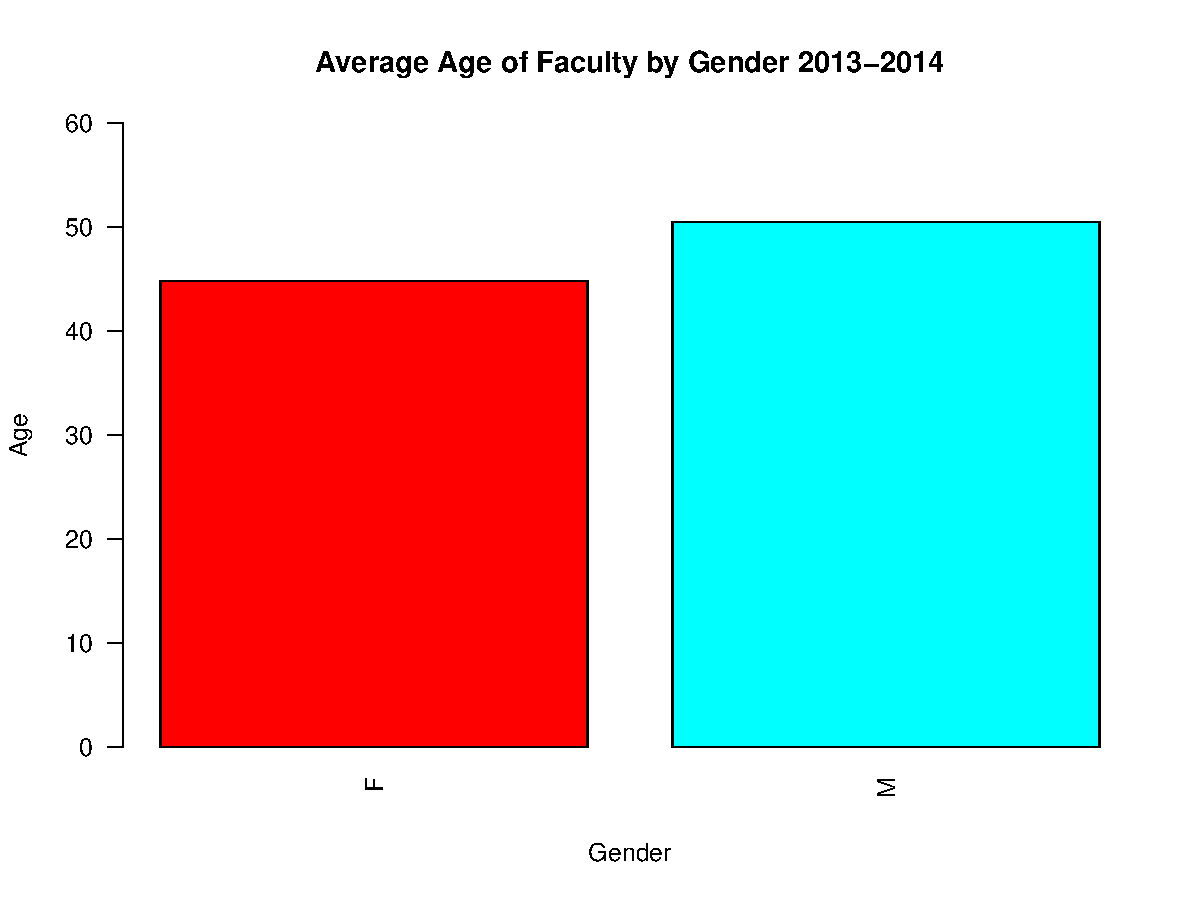
\includegraphics[width=\maxwidth]{figure/unnamed-chunk-11-10} 
\begin{kframe}\begin{verbatim}
## [1] "Average Age by Gender 2013-2014:"
##    F    M 
## 44.8 50.5
\end{verbatim}
\end{kframe}
\end{knitrout}
\bigskip
An interesting aspect of this analysis of the course catalogs is that the male faculty has been signficantly older than the female faculty for the past 10 years. In addtion, both the male and female faculty average age has increased over the past 10 years, with the female faculty aging by 2 years and the male faculty aging by 3 years. It is also interesting to note that the gap in average age between the female and male faculty has increased, with the gap in 2004-2005 being 3.4 years and in 2013-204 the gap was 5.3 years.

\bigskip
How High is the Correlation between Age and Year of Terminal Degree.

\begin{knitrout}
\definecolor{shadecolor}{rgb}{0.969, 0.969, 0.969}\color{fgcolor}
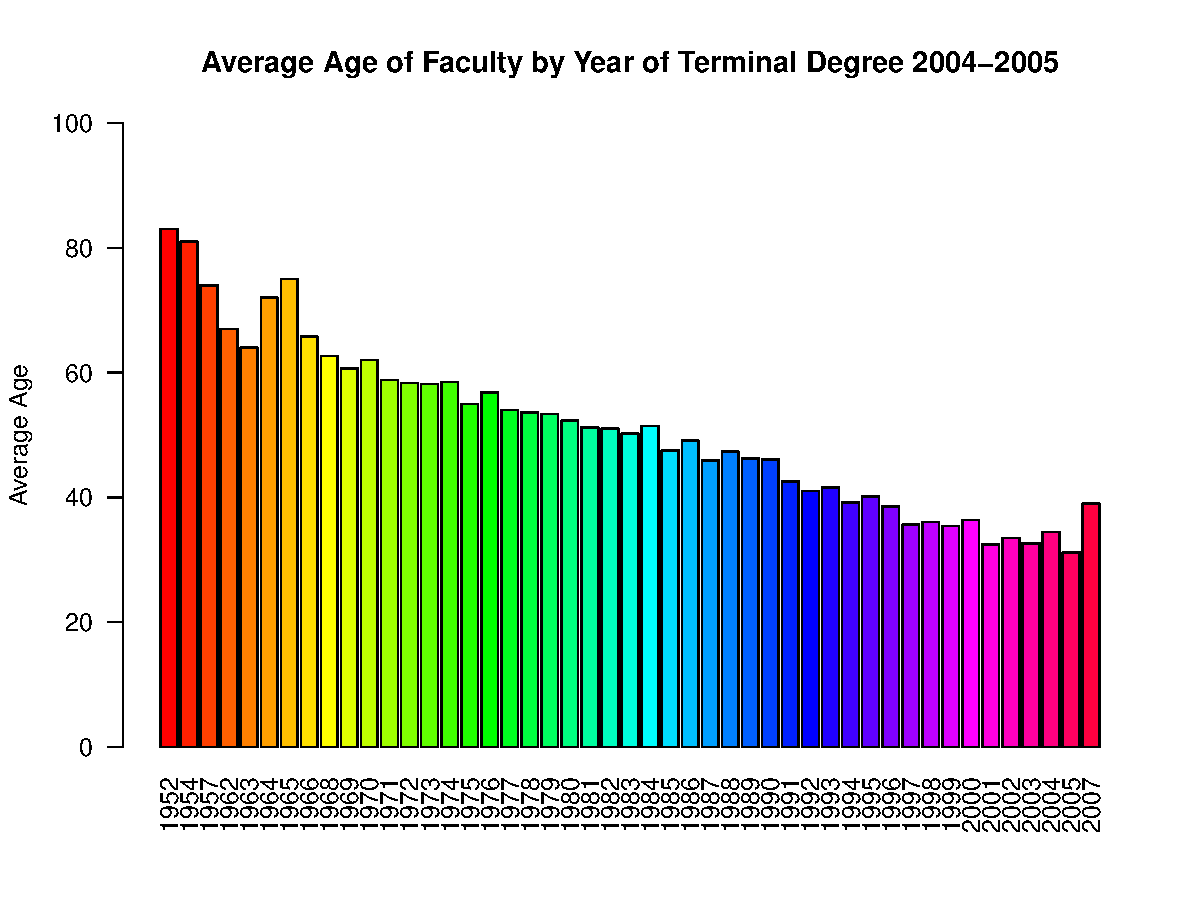
\includegraphics[width=\maxwidth]{figure/unnamed-chunk-12-1} 
\begin{kframe}\begin{verbatim}
## [1] "Correlation Between Age and Year of Terminal Degree 2004-2005"
## [1] -0.93
\end{verbatim}
\end{kframe}
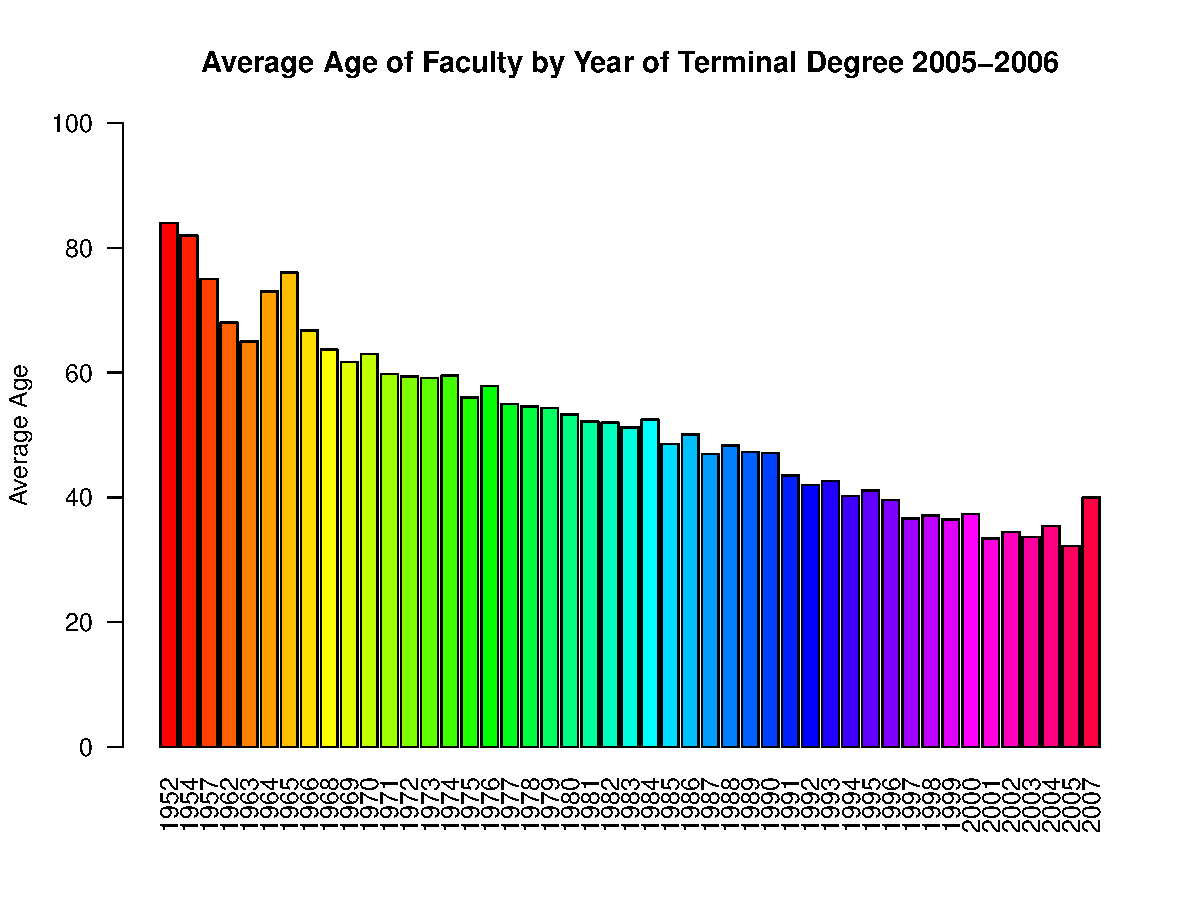
\includegraphics[width=\maxwidth]{figure/unnamed-chunk-12-2} 
\begin{kframe}\begin{verbatim}
## [1] "Correlation Between Age and Year of Terminal Degree 2005-2006"
## [1] -0.93
\end{verbatim}
\end{kframe}
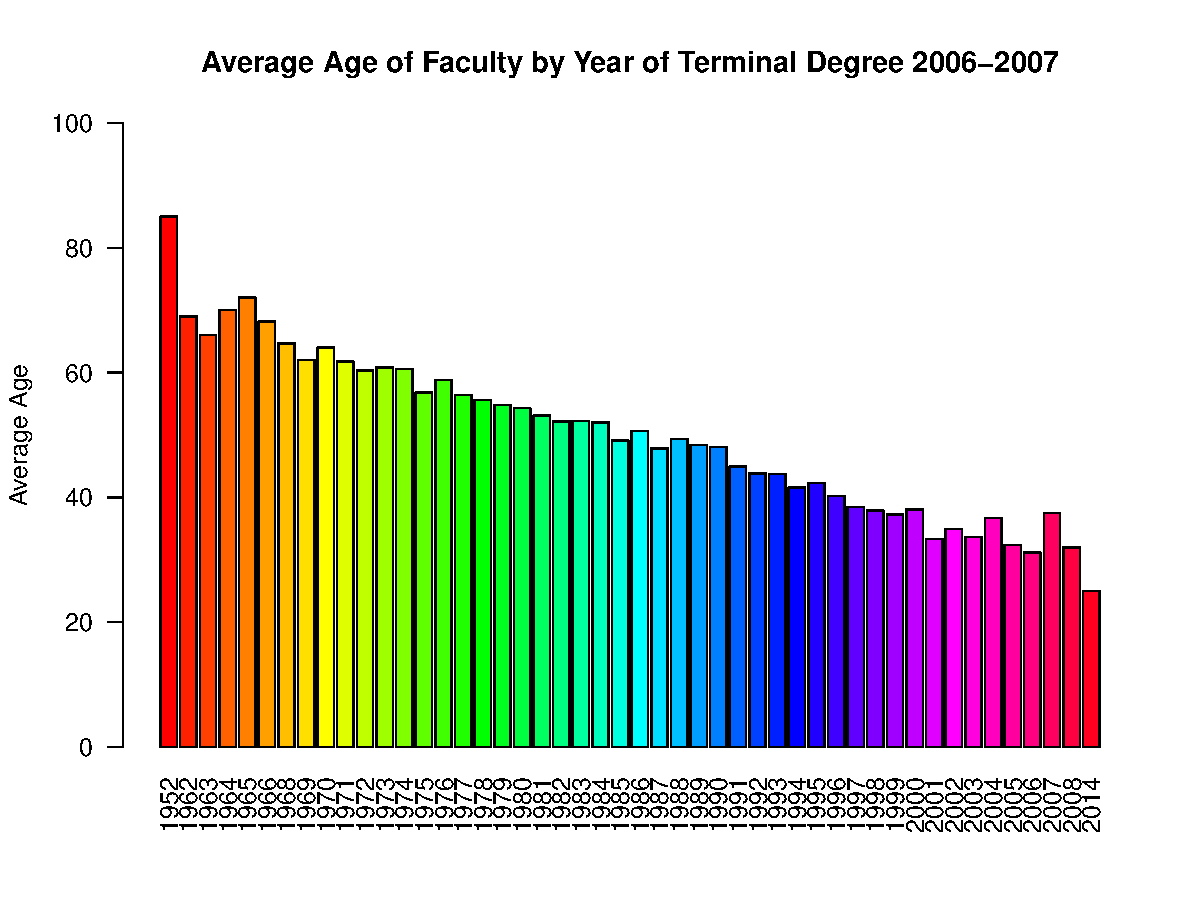
\includegraphics[width=\maxwidth]{figure/unnamed-chunk-12-3} 
\begin{kframe}\begin{verbatim}
## [1] "Correlation Between Age and Year of Terminal Degree 2006-2007"
## [1] -0.93
\end{verbatim}
\end{kframe}
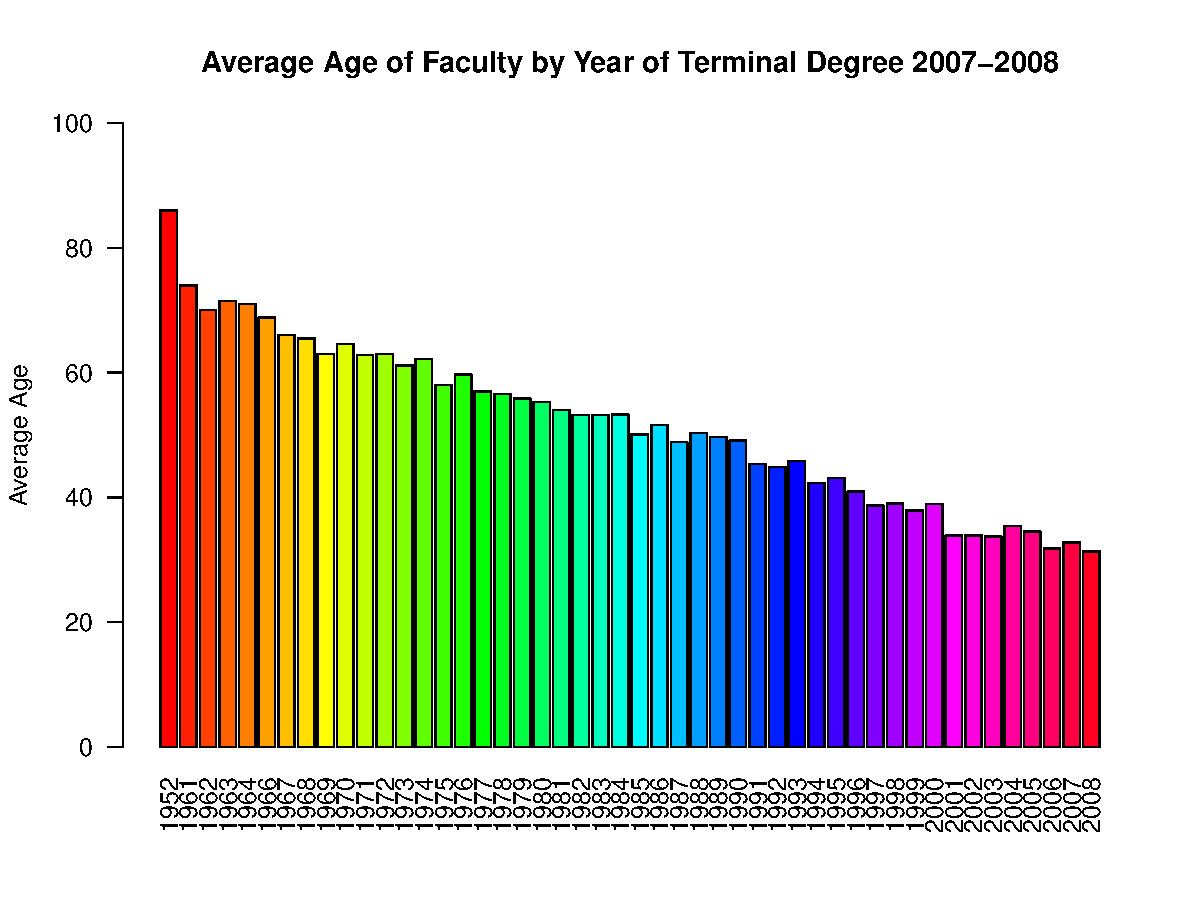
\includegraphics[width=\maxwidth]{figure/unnamed-chunk-12-4} 
\begin{kframe}\begin{verbatim}
## [1] "Correlation Between Age and Year of Terminal Degree 2007-2008"
## [1] -0.94
\end{verbatim}
\end{kframe}
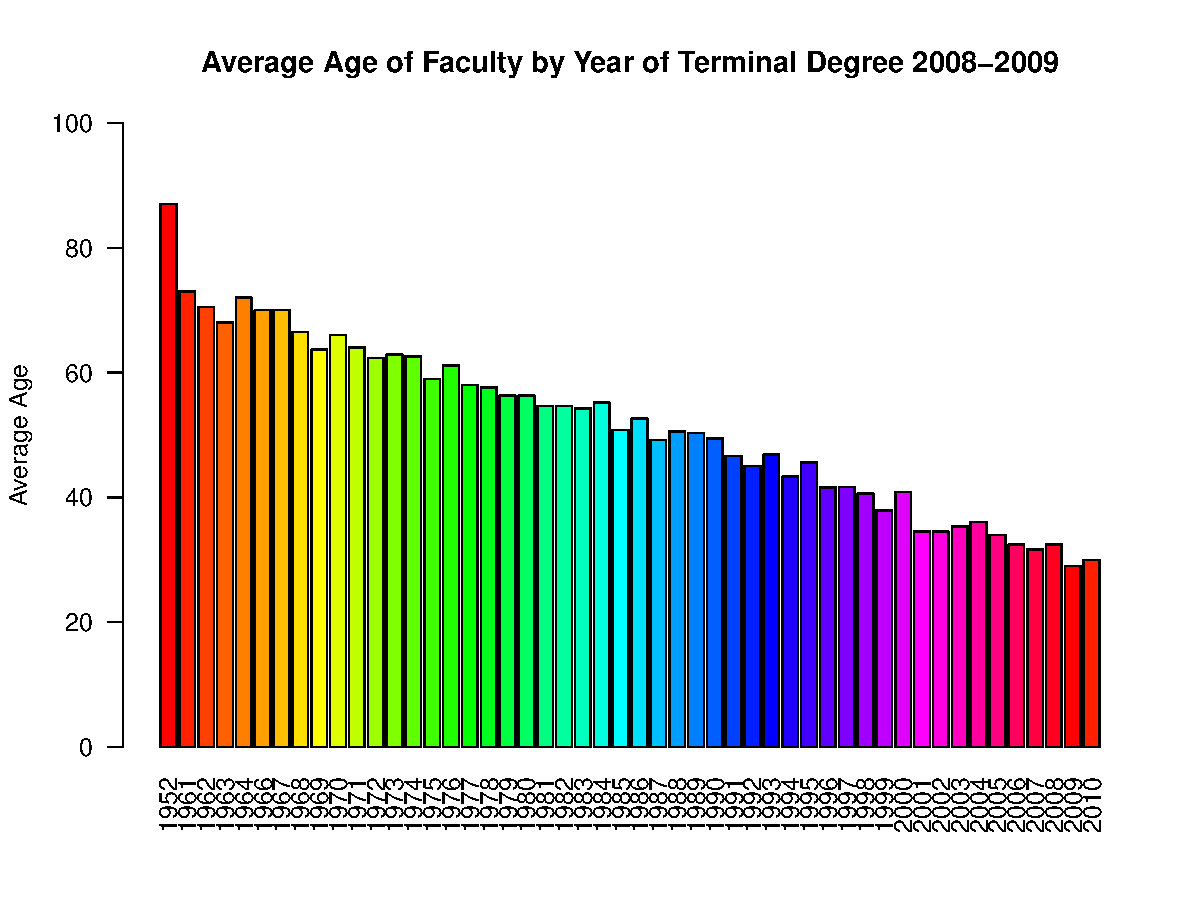
\includegraphics[width=\maxwidth]{figure/unnamed-chunk-12-5} 
\begin{kframe}\begin{verbatim}
## [1] "Correlation Between Age and Year of Terminal Degree 2008-2009"
## [1] -0.93
\end{verbatim}
\end{kframe}
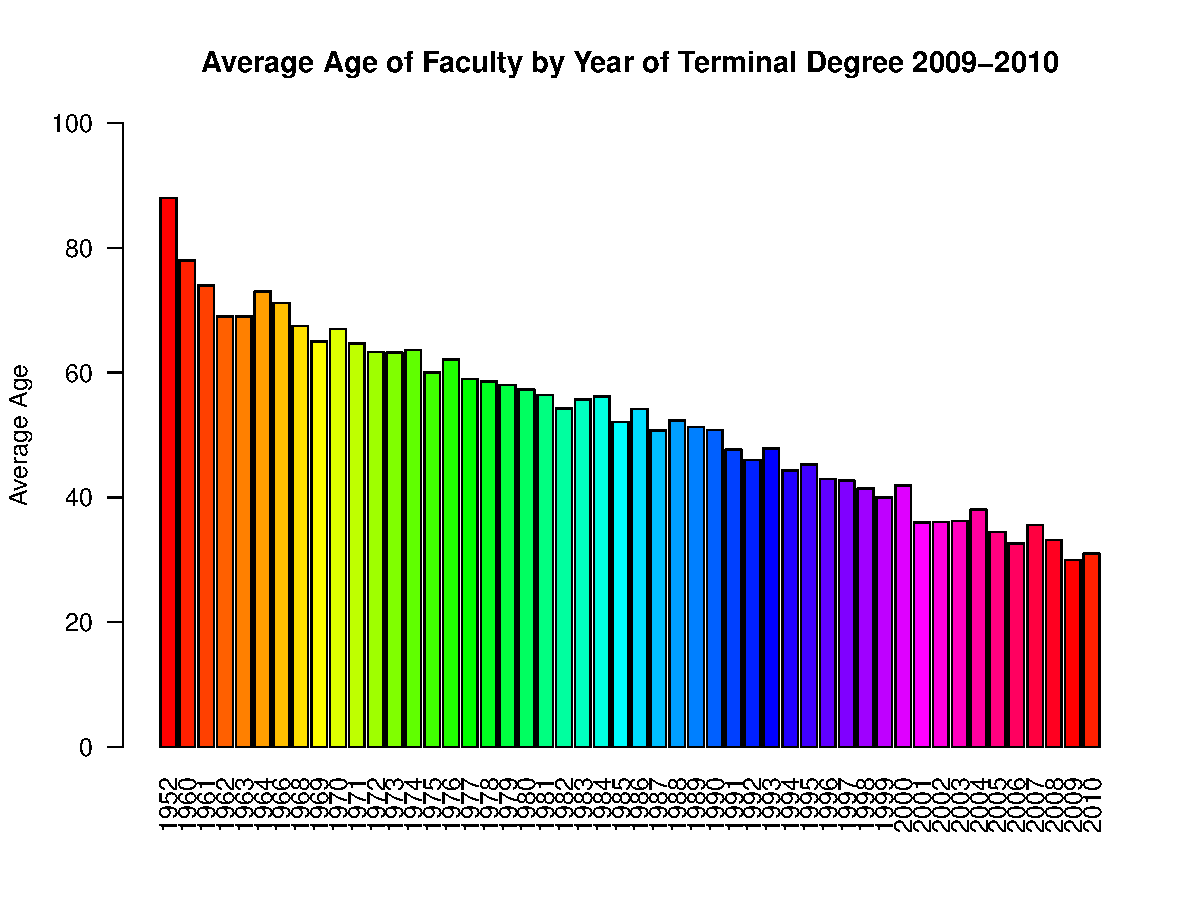
\includegraphics[width=\maxwidth]{figure/unnamed-chunk-12-6} 
\begin{kframe}\begin{verbatim}
## [1] "Correlation Between Age and Year of Terminal Degree 2009-2010"
## [1] -0.94
\end{verbatim}
\end{kframe}
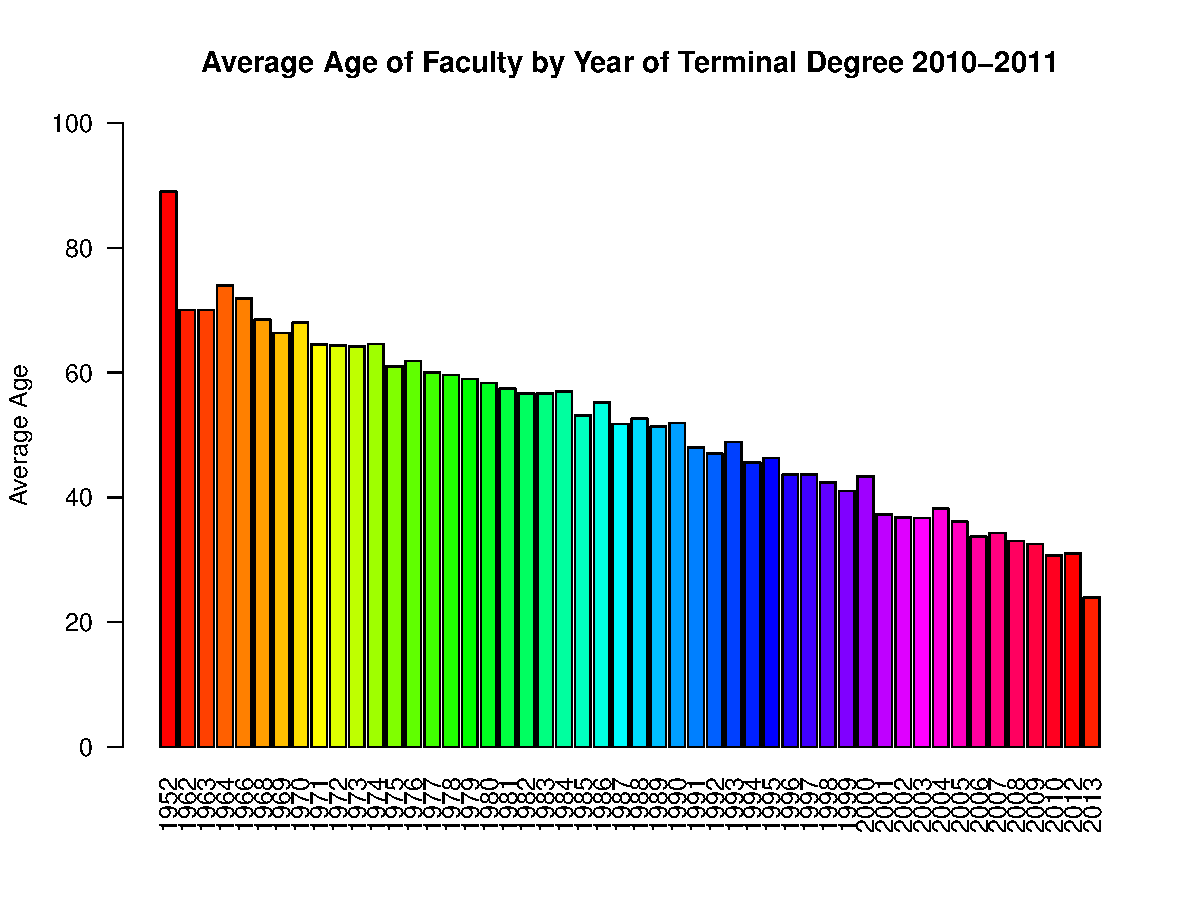
\includegraphics[width=\maxwidth]{figure/unnamed-chunk-12-7} 
\begin{kframe}\begin{verbatim}
## [1] "Correlation Between Age and Year of Terminal Degree 2010-2011"
## [1] -0.95
\end{verbatim}
\end{kframe}
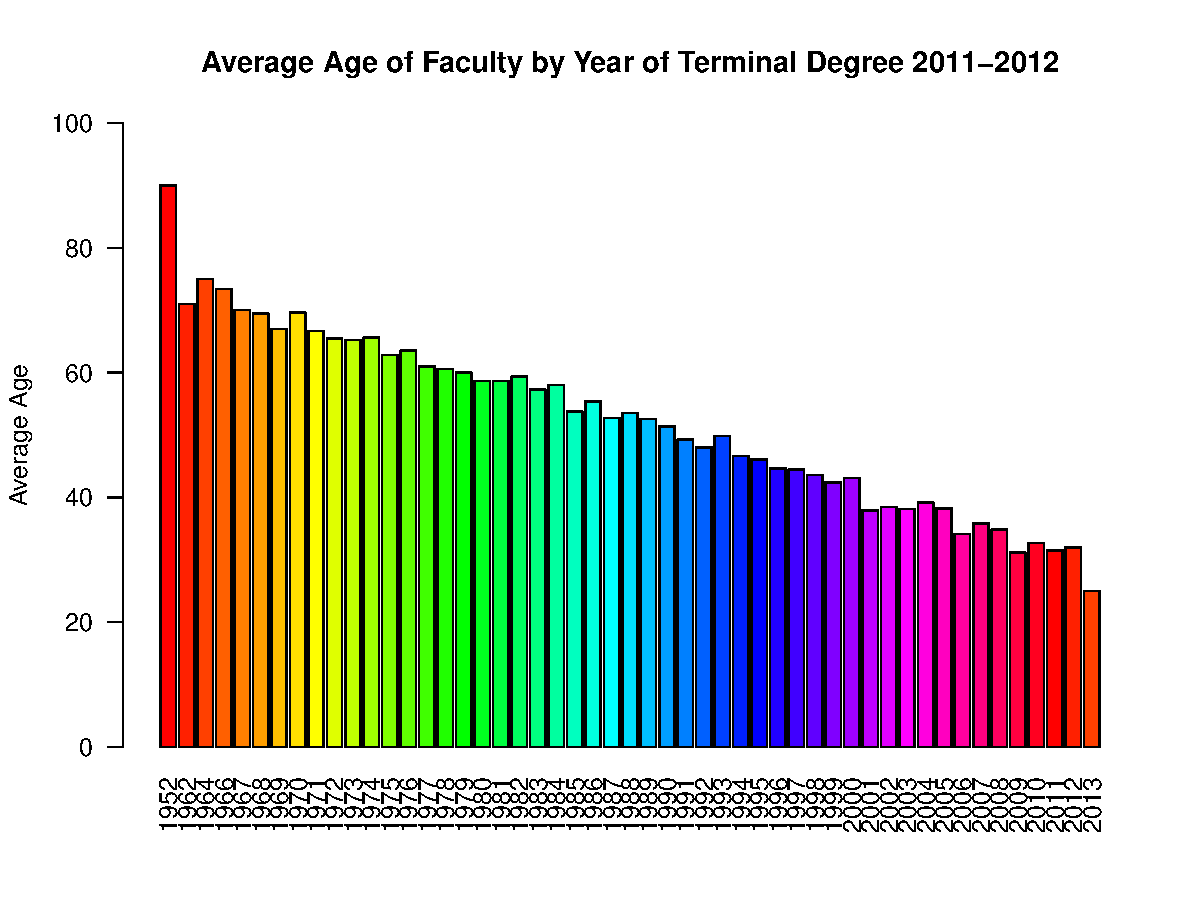
\includegraphics[width=\maxwidth]{figure/unnamed-chunk-12-8} 
\begin{kframe}\begin{verbatim}
## [1] "Correlation Between Age and Year of Terminal Degree 2011-2012"
## [1] -0.95
\end{verbatim}
\end{kframe}
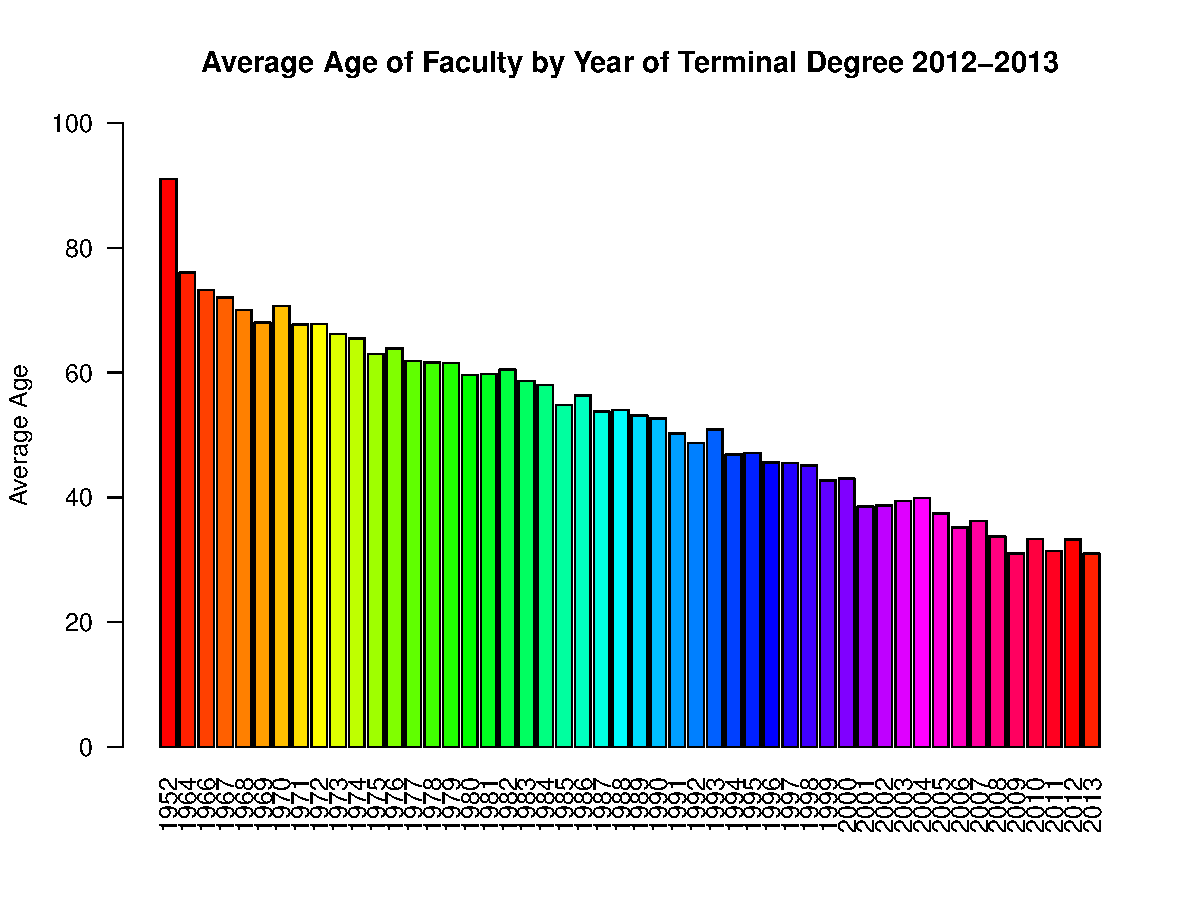
\includegraphics[width=\maxwidth]{figure/unnamed-chunk-12-9} 
\begin{kframe}\begin{verbatim}
## [1] "Correlation Between Age and Year of Terminal Degree 2012-2013"
## [1] -0.95
\end{verbatim}
\end{kframe}
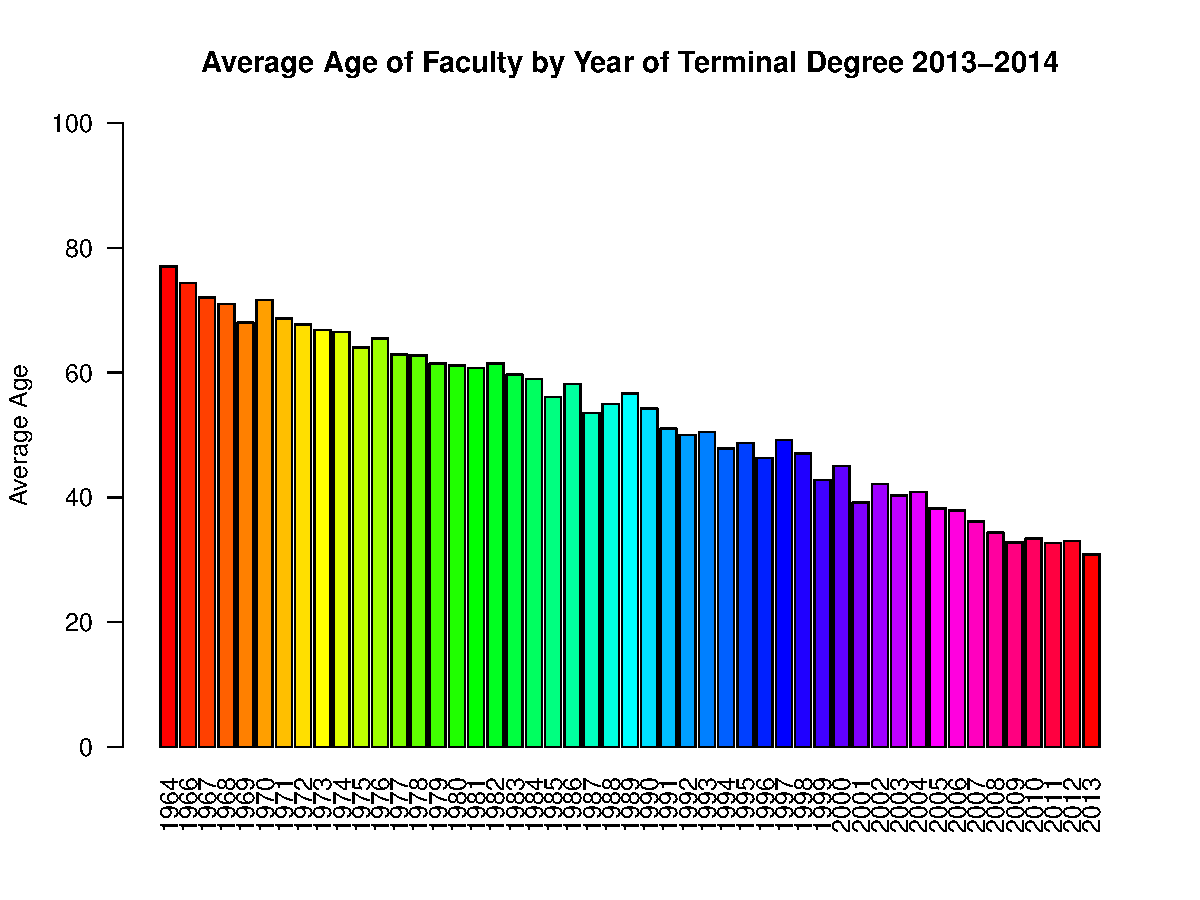
\includegraphics[width=\maxwidth]{figure/unnamed-chunk-12-10} 
\begin{kframe}\begin{verbatim}
## [1] "Correlation Between Age and Year of Terminal Degree 2013-2014"
## [1] -0.94
\end{verbatim}
\end{kframe}
\end{knitrout}

\bigskip
Do certain departments require more time to earn a PhD in than others?

\begin{knitrout}
\definecolor{shadecolor}{rgb}{0.969, 0.969, 0.969}\color{fgcolor}
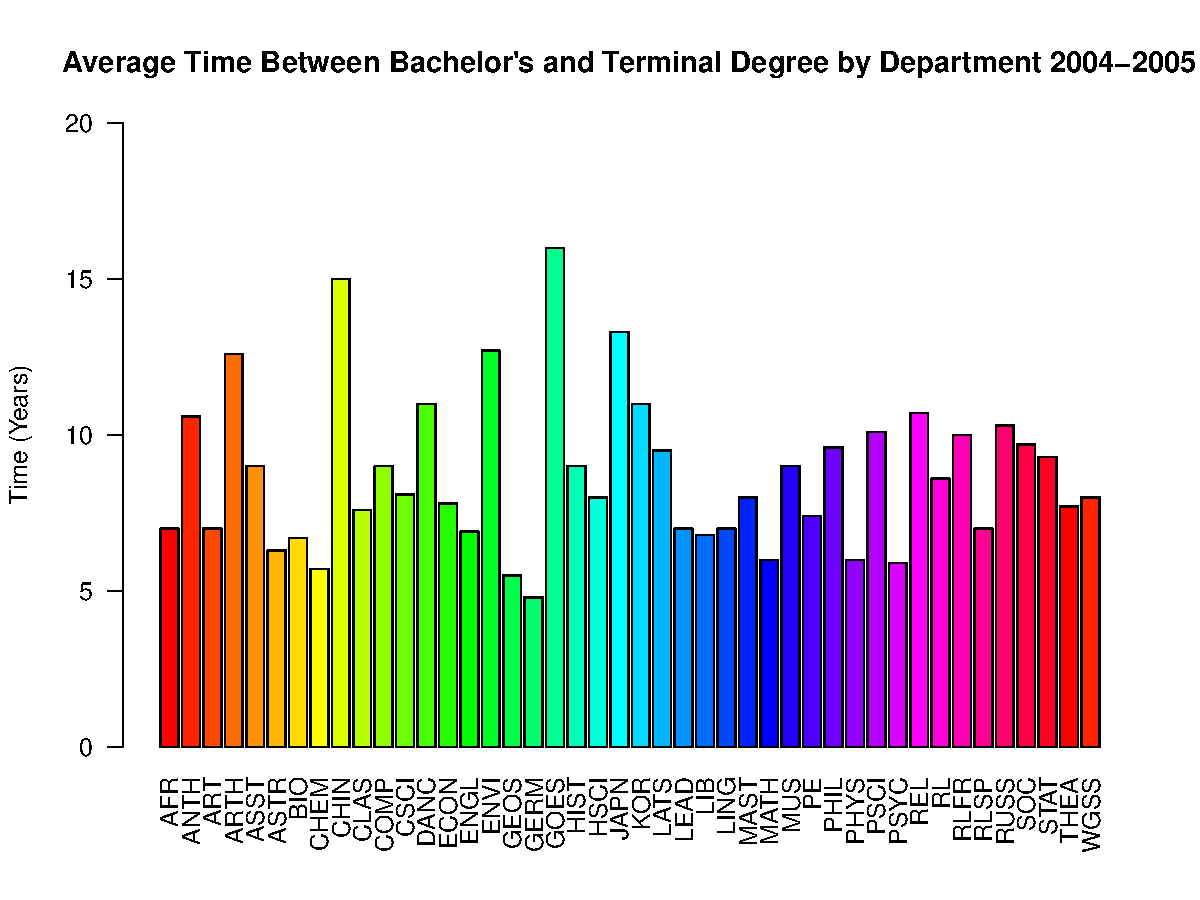
\includegraphics[width=\maxwidth]{figure/unnamed-chunk-13-1} 
\begin{kframe}\begin{verbatim}
## [1] "Avg Time b/w Bachelor's and Terminal Degree by Dept 2004-2005"
##  AFR ANTH  ART ARTH ASST ASTR  BIO CHEM CHIN CLAS COMP CSCI 
##  7.0 10.6  7.0 12.6  9.0  6.3  6.7  5.7 15.0  7.6  9.0  8.1 
## DANC ECON ENGL ENVI GEOS GERM GOES HIST HSCI JAPN  KOR LATS 
## 11.0  7.8  6.9 12.7  5.5  4.8 16.0  9.0  8.0 13.3 11.0  9.5 
## LEAD  LIB LING MAST MATH  MUS   PE PHIL PHYS PSCI PSYC  REL 
##  7.0  6.8  7.0  8.0  6.0  9.0  7.4  9.6  6.0 10.1  5.9 10.7 
##   RL RLFR RLSP RUSS  SOC STAT THEA WGSS 
##  8.6 10.0  7.0 10.3  9.7  9.3  7.7  8.0
\end{verbatim}
\end{kframe}
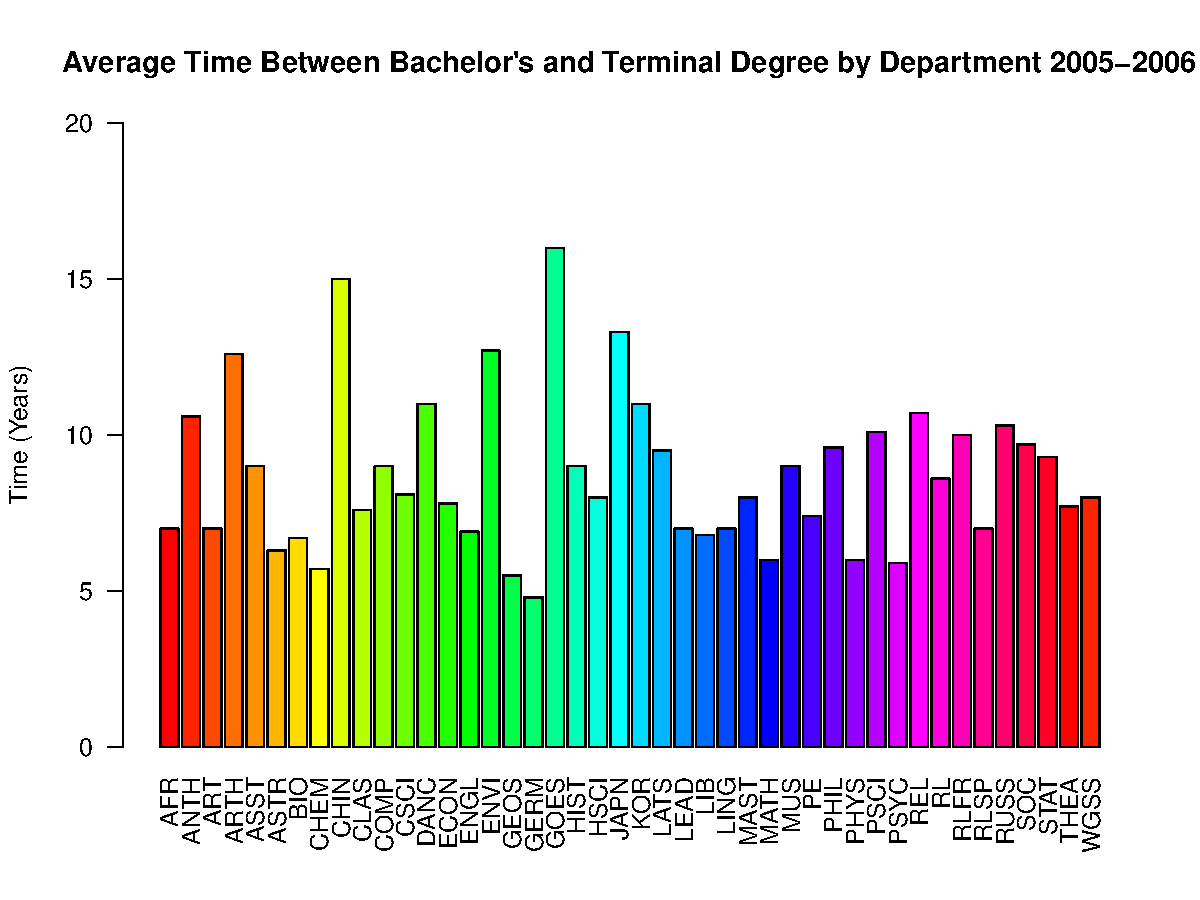
\includegraphics[width=\maxwidth]{figure/unnamed-chunk-13-2} 
\begin{kframe}\begin{verbatim}
## [1] "Avg Time b/w Bachelor's and Terminal Degree by Dept 2005-2006"
##  AFR ANTH  ART ARTH ASST ASTR  BIO CHEM CHIN CLAS COMP CSCI 
##  7.0 10.6  7.0 12.6  9.0  6.3  6.7  5.7 15.0  7.6  9.0  8.1 
## DANC ECON ENGL ENVI GEOS GERM GOES HIST HSCI JAPN  KOR LATS 
## 11.0  7.8  6.9 12.7  5.5  4.8 16.0  9.0  8.0 13.3 11.0  9.5 
## LEAD  LIB LING MAST MATH  MUS   PE PHIL PHYS PSCI PSYC  REL 
##  7.0  6.8  7.0  8.0  6.0  9.0  7.4  9.6  6.0 10.1  5.9 10.7 
##   RL RLFR RLSP RUSS  SOC STAT THEA WGSS 
##  8.6 10.0  7.0 10.3  9.7  9.3  7.7  8.0
\end{verbatim}
\end{kframe}
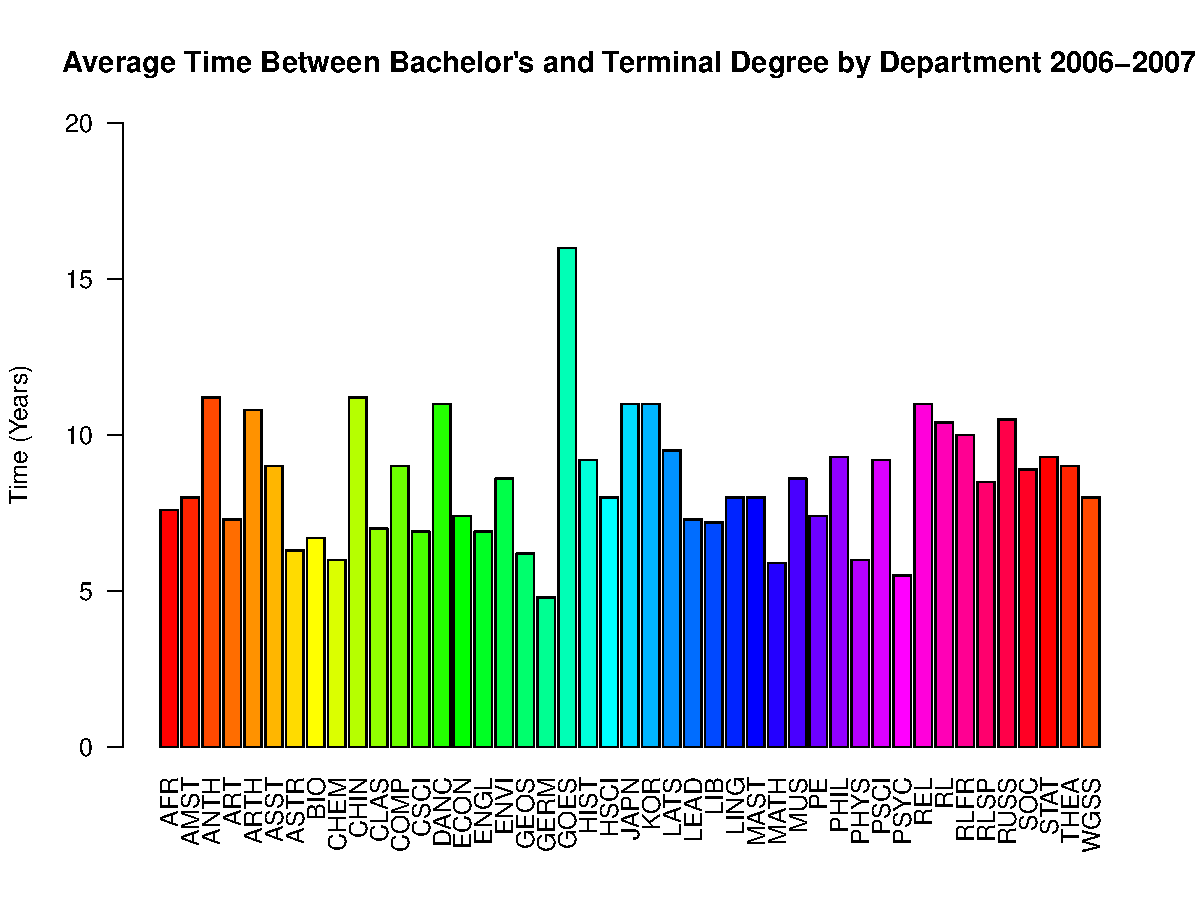
\includegraphics[width=\maxwidth]{figure/unnamed-chunk-13-3} 
\begin{kframe}\begin{verbatim}
## [1] "Avg Time b/w Bachelor's and Terminal Degree by Dept 2006-2007"
##  AFR AMST ANTH  ART ARTH ASST ASTR  BIO CHEM CHIN CLAS COMP 
##  7.6  8.0 11.2  7.3 10.8  9.0  6.3  6.7  6.0 11.2  7.0  9.0 
## CSCI DANC ECON ENGL ENVI GEOS GERM GOES HIST HSCI JAPN  KOR 
##  6.9 11.0  7.4  6.9  8.6  6.2  4.8 16.0  9.2  8.0 11.0 11.0 
## LATS LEAD  LIB LING MAST MATH  MUS   PE PHIL PHYS PSCI PSYC 
##  9.5  7.3  7.2  8.0  8.0  5.9  8.6  7.4  9.3  6.0  9.2  5.5 
##  REL   RL RLFR RLSP RUSS  SOC STAT THEA WGSS 
## 11.0 10.4 10.0  8.5 10.5  8.9  9.3  9.0  8.0
\end{verbatim}
\end{kframe}
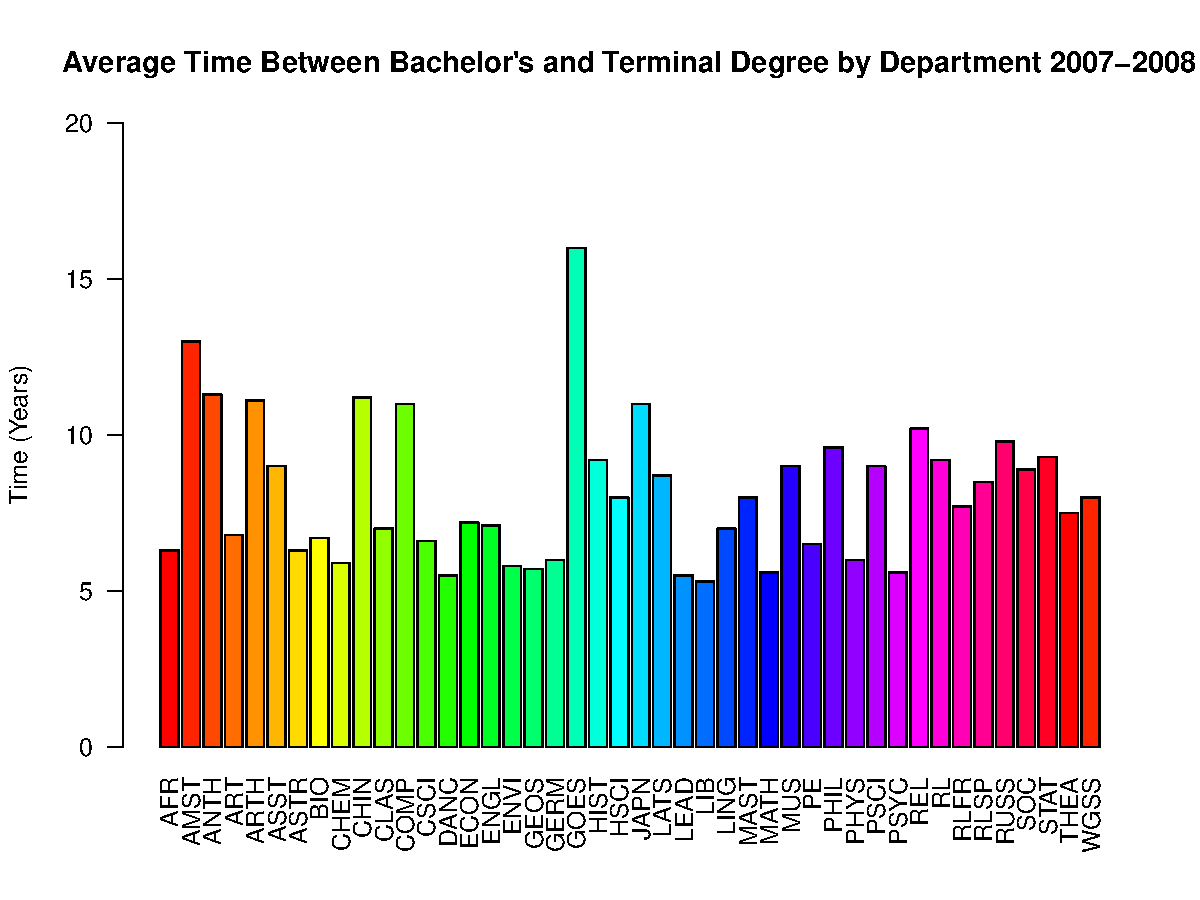
\includegraphics[width=\maxwidth]{figure/unnamed-chunk-13-4} 
\begin{kframe}\begin{verbatim}
## [1] "Avg Time b/w Bachelor's and Terminal Degree by Dept 2007-2008"
##  AFR AMST ANTH  ART ARTH ASST ASTR  BIO CHEM CHIN CLAS COMP 
##  6.3 13.0 11.3  6.8 11.1  9.0  6.3  6.7  5.9 11.2  7.0 11.0 
## CSCI DANC ECON ENGL ENVI GEOS GERM GOES HIST HSCI JAPN LATS 
##  6.6  5.5  7.2  7.1  5.8  5.7  6.0 16.0  9.2  8.0 11.0  8.7 
## LEAD  LIB LING MAST MATH  MUS   PE PHIL PHYS PSCI PSYC  REL 
##  5.5  5.3  7.0  8.0  5.6  9.0  6.5  9.6  6.0  9.0  5.6 10.2 
##   RL RLFR RLSP RUSS  SOC STAT THEA WGSS 
##  9.2  7.7  8.5  9.8  8.9  9.3  7.5  8.0
\end{verbatim}
\end{kframe}
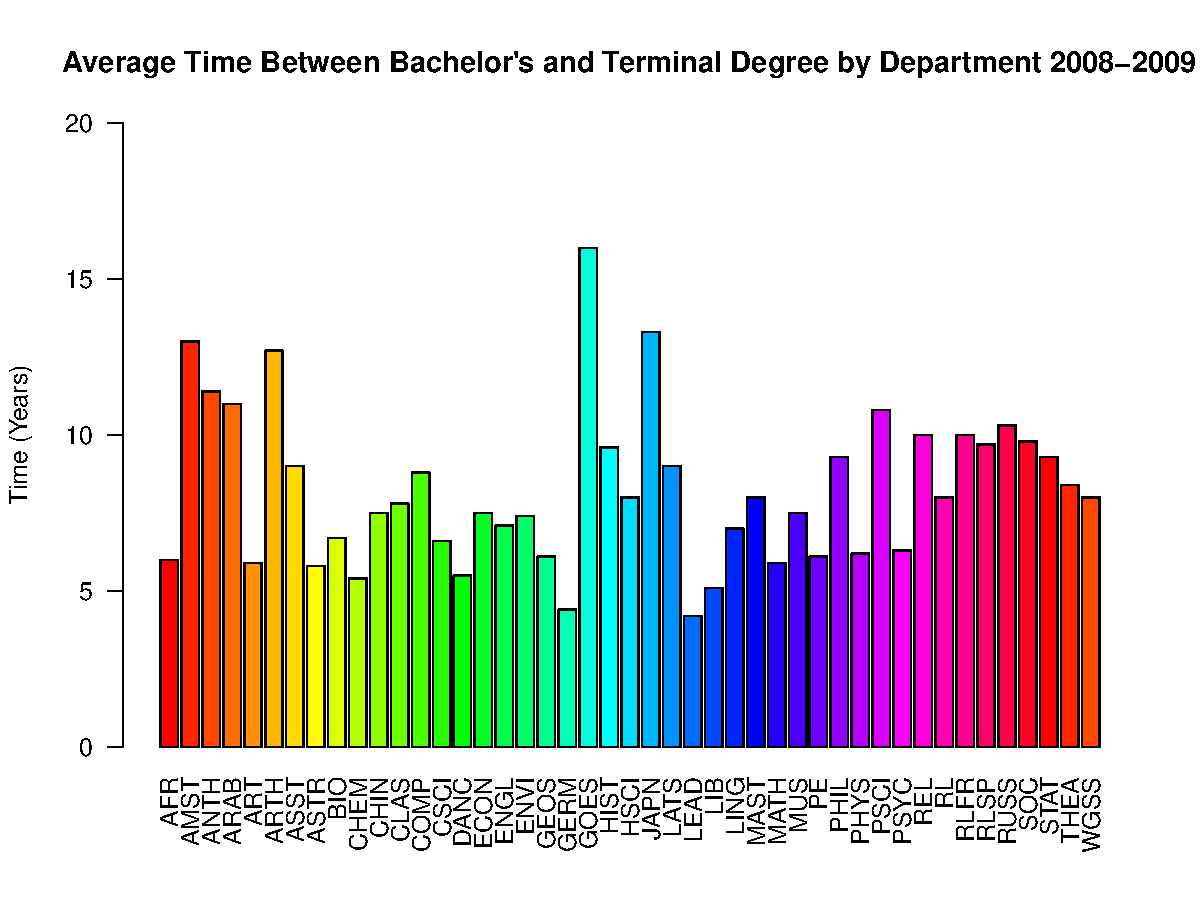
\includegraphics[width=\maxwidth]{figure/unnamed-chunk-13-5} 
\begin{kframe}\begin{verbatim}
## [1] "Avg Time b/w Bachelor's and Terminal Degree by Dept 2008-2009"
##  AFR AMST ANTH ARAB  ART ARTH ASST ASTR  BIO CHEM CHIN CLAS 
##  6.0 13.0 11.4 11.0  5.9 12.7  9.0  5.8  6.7  5.4  7.5  7.8 
## COMP CSCI DANC ECON ENGL ENVI GEOS GERM GOES HIST HSCI JAPN 
##  8.8  6.6  5.5  7.5  7.1  7.4  6.1  4.4 16.0  9.6  8.0 13.3 
## LATS LEAD  LIB LING MAST MATH  MUS   PE PHIL PHYS PSCI PSYC 
##  9.0  4.2  5.1  7.0  8.0  5.9  7.5  6.1  9.3  6.2 10.8  6.3 
##  REL   RL RLFR RLSP RUSS  SOC STAT THEA WGSS 
## 10.0  8.0 10.0  9.7 10.3  9.8  9.3  8.4  8.0
\end{verbatim}
\end{kframe}
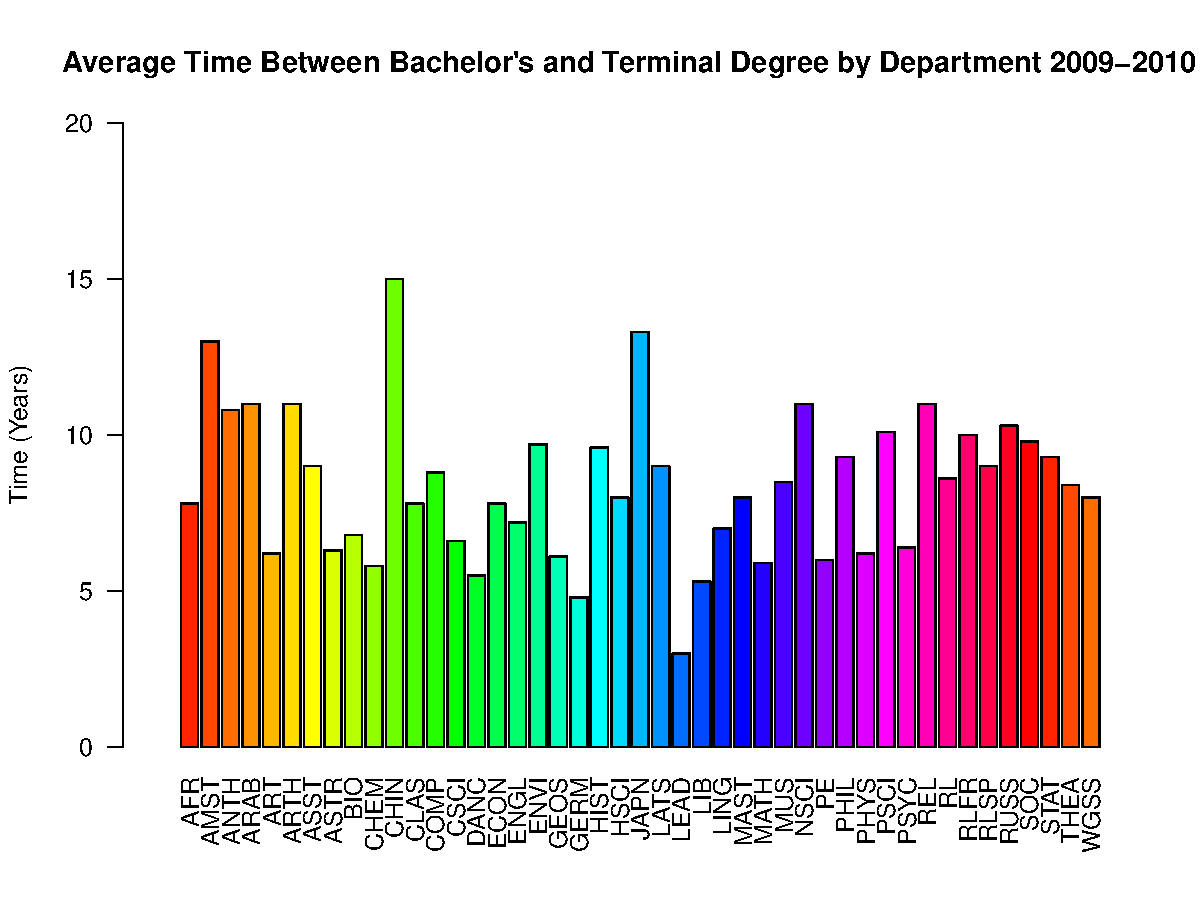
\includegraphics[width=\maxwidth]{figure/unnamed-chunk-13-6} 
\begin{kframe}\begin{verbatim}
## [1] "Avg Time b/w Bachelor's and Terminal Degree by Dept 2009-2010"
##       AFR AMST ANTH ARAB  ART ARTH ASST ASTR  BIO CHEM CHIN 
##   NA  7.8 13.0 10.8 11.0  6.2 11.0  9.0  6.3  6.8  5.8 15.0 
## CLAS COMP CSCI DANC ECON ENGL ENVI GEOS GERM HIST HSCI JAPN 
##  7.8  8.8  6.6  5.5  7.8  7.2  9.7  6.1  4.8  9.6  8.0 13.3 
## LATS LEAD  LIB LING MAST MATH  MUS NSCI   PE PHIL PHYS PSCI 
##  9.0  3.0  5.3  7.0  8.0  5.9  8.5 11.0  6.0  9.3  6.2 10.1 
## PSYC  REL   RL RLFR RLSP RUSS  SOC STAT THEA WGSS 
##  6.4 11.0  8.6 10.0  9.0 10.3  9.8  9.3  8.4  8.0
\end{verbatim}
\end{kframe}
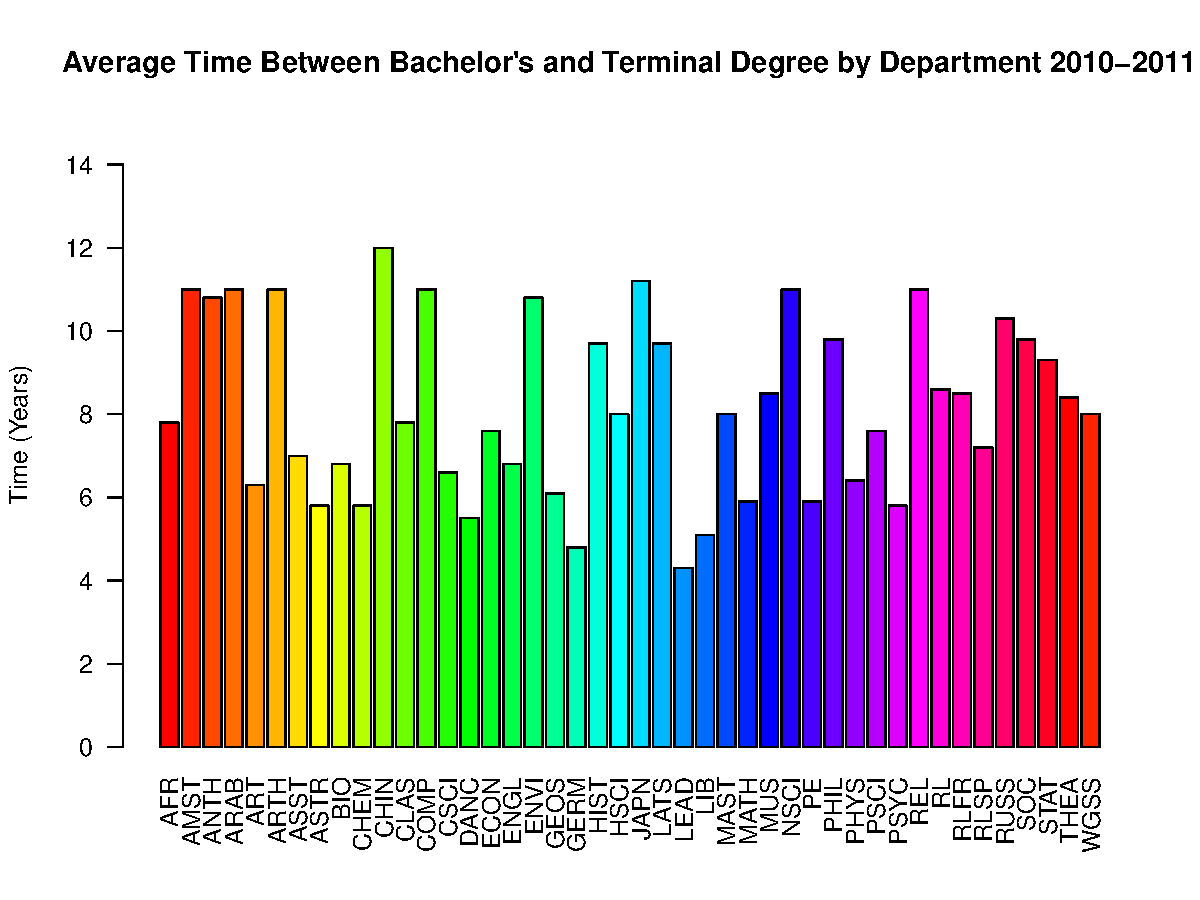
\includegraphics[width=\maxwidth]{figure/unnamed-chunk-13-7} 
\begin{kframe}\begin{verbatim}
## [1] "Avg Time b/w Bachelor's and Terminal Degree by Dept 2010-2011"
##  AFR AMST ANTH ARAB  ART ARTH ASST ASTR  BIO CHEM CHIN CLAS 
##  7.8 11.0 10.8 11.0  6.3 11.0  7.0  5.8  6.8  5.8 12.0  7.8 
## COMP CSCI DANC ECON ENGL ENVI GEOS GERM HIST HSCI JAPN LATS 
## 11.0  6.6  5.5  7.6  6.8 10.8  6.1  4.8  9.7  8.0 11.2  9.7 
## LEAD  LIB MAST MATH  MUS NSCI   PE PHIL PHYS PSCI PSYC  REL 
##  4.3  5.1  8.0  5.9  8.5 11.0  5.9  9.8  6.4  7.6  5.8 11.0 
##   RL RLFR RLSP RUSS  SOC STAT THEA WGSS 
##  8.6  8.5  7.2 10.3  9.8  9.3  8.4  8.0
\end{verbatim}
\end{kframe}
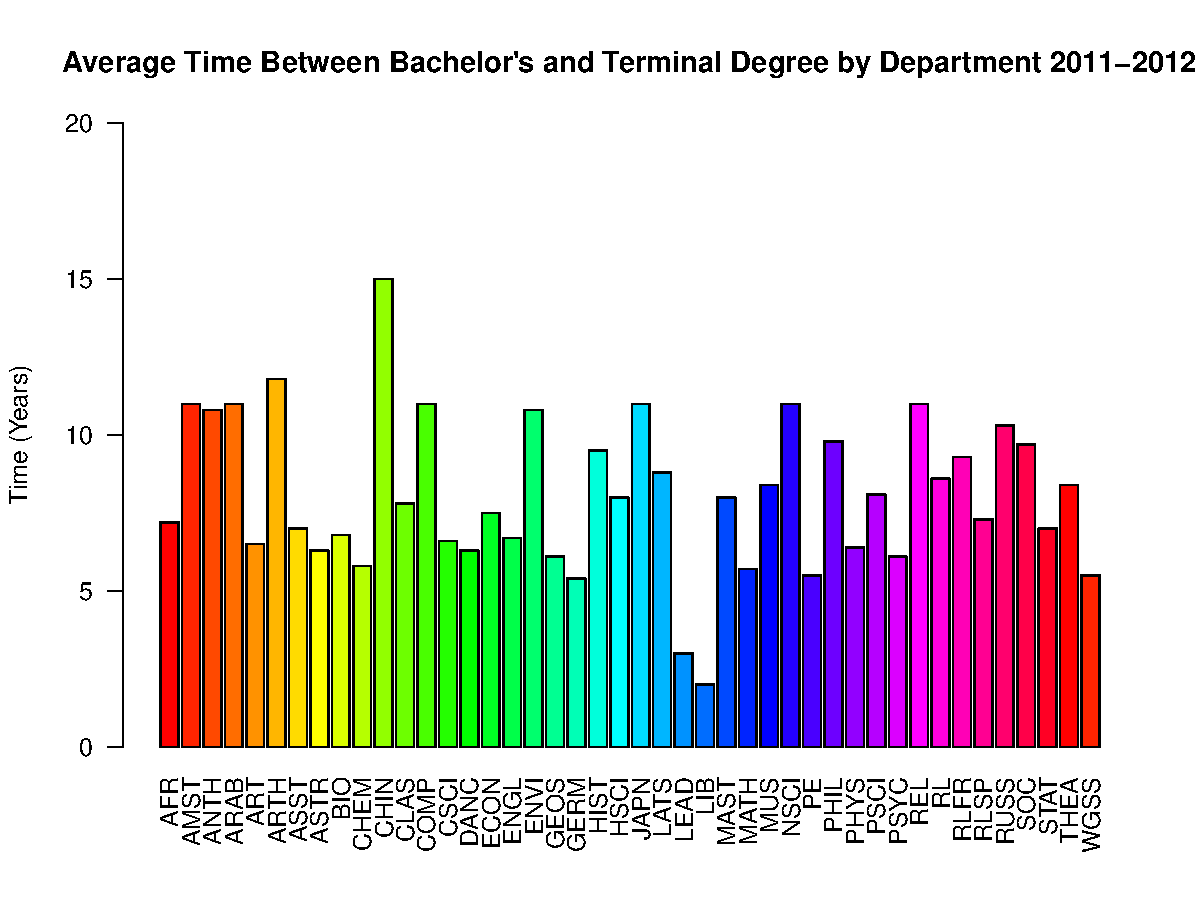
\includegraphics[width=\maxwidth]{figure/unnamed-chunk-13-8} 
\begin{kframe}\begin{verbatim}
## [1] "Avg Time b/w Bachelor's and Terminal Degree by Dept 2011-2012"
##  AFR AMST ANTH ARAB  ART ARTH ASST ASTR  BIO CHEM CHIN CLAS 
##  7.2 11.0 10.8 11.0  6.5 11.8  7.0  6.3  6.8  5.8 15.0  7.8 
## COMP CSCI DANC ECON ENGL ENVI GEOS GERM HIST HSCI JAPN LATS 
## 11.0  6.6  6.3  7.5  6.7 10.8  6.1  5.4  9.5  8.0 11.0  8.8 
## LEAD  LIB MAST MATH  MUS NSCI   PE PHIL PHYS PSCI PSYC  REL 
##  3.0  2.0  8.0  5.7  8.4 11.0  5.5  9.8  6.4  8.1  6.1 11.0 
##   RL RLFR RLSP RUSS  SOC STAT THEA WGSS 
##  8.6  9.3  7.3 10.3  9.7  7.0  8.4  5.5
\end{verbatim}
\end{kframe}
\includegraphics[width=\maxwidth]{figure/unnamed-chunk-13-9} 
\begin{kframe}\begin{verbatim}
## [1] "Avg Time b/w Bachelor's and Terminal Degree by Dept 2012-2013"
##  AFR AMST ANTH ARAB  ART ARTH ASST ASTR  BIO CHEM CHIN CLAS 
##  7.2 12.0 10.8 11.0  7.1  9.8  9.0  5.8  6.8  5.4 15.0  8.2 
## COMP CSCI DANC ECON ENGL ENVI GEOS GERM HIST HSCI JAPN LATS 
## 11.0  6.6  5.3  7.4  7.1 10.8  6.4  5.4  9.5  8.0 11.6  9.7 
## LEAD  LIB MAST MATH  MUS NSCI   PE PHIL PHYS PSCI PSYC  REL 
##  4.3  2.0  8.0  5.8  6.7 11.0  5.2  9.5  6.2  8.0  5.8 10.0 
##   RL RLFR RLSP RUSS  SOC STAT THEA WGSS 
##  9.2 10.2  9.3 10.0  7.8  5.8  8.6  7.7
\end{verbatim}
\end{kframe}
\includegraphics[width=\maxwidth]{figure/unnamed-chunk-13-10} 
\begin{kframe}\begin{verbatim}
## [1] "Avg Time b/w Bachelor's and Terminal Degree by Dept 2013-2014"
##       AFR AMST ANTH ARAB  ART ARTH ASST ASTR  BIO CHEM CHIN 
##  0.0  9.8 13.0 10.8 13.5  7.7  9.1  9.0  5.8  7.2  5.7 10.8 
## CLAS COMP CSCI DANC ECON ENGL ENVI GEOS GERM HIST HSCI INST 
##  7.9 12.0  6.6  6.0  6.8  7.6 10.8  7.6  5.2  9.9  8.0  5.0 
## JAPN LATS LEAD MAST MATH  MUS NSCI   PE PHIL PHYS PSCI PSYC 
##  9.8  8.0  7.0  8.0  5.1  6.6 11.0  4.9  9.5  6.1  9.4  6.0 
##  REL   RL RLFR RLSP RUSS  SOC STAT THEA WGSS 
## 11.0  7.9 11.3  8.3 10.3  8.8  7.0  8.4 10.0
\end{verbatim}
\end{kframe}
\end{knitrout}

\bigskip
Has the actual, non bin Distribution of Ages changed significantly over the last 10 years with summary stats:

\begin{knitrout}
\definecolor{shadecolor}{rgb}{0.969, 0.969, 0.969}\color{fgcolor}
\includegraphics[width=\maxwidth]{figure/unnamed-chunk-14-1} 

\end{knitrout}

\begin{knitrout}
\definecolor{shadecolor}{rgb}{0.969, 0.969, 0.969}\color{fgcolor}\begin{kframe}
\begin{verbatim}
## [1] "Summary Statistics with Standard Deviation 2004-2005"
##    Min. 1st Qu.  Median    Mean 3rd Qu.    Max. 
##   24.00   36.00   45.00   45.05   53.00   83.00
## [1] "Standard Deviation:10.9"
\end{verbatim}
\end{kframe}
\end{knitrout}

\begin{knitrout}
\definecolor{shadecolor}{rgb}{0.969, 0.969, 0.969}\color{fgcolor}
\includegraphics[width=\maxwidth]{figure/unnamed-chunk-16-1} 

\end{knitrout}

\begin{knitrout}
\definecolor{shadecolor}{rgb}{0.969, 0.969, 0.969}\color{fgcolor}\begin{kframe}
\begin{verbatim}
## [1] "Summary Statistics with Standard Deviation 2005-2006"
##    Min. 1st Qu.  Median    Mean 3rd Qu.    Max. 
##   25.00   37.00   46.00   46.03   54.00   84.00
## [1] "Standard Deviation:10.89"
\end{verbatim}
\end{kframe}
\end{knitrout}


\begin{knitrout}
\definecolor{shadecolor}{rgb}{0.969, 0.969, 0.969}\color{fgcolor}
\includegraphics[width=\maxwidth]{figure/unnamed-chunk-18-1} 

\end{knitrout}

\begin{knitrout}
\definecolor{shadecolor}{rgb}{0.969, 0.969, 0.969}\color{fgcolor}\begin{kframe}
\begin{verbatim}
## [1] "Summary Statistics with Standard Deviation 2006-2007"
##    Min. 1st Qu.  Median    Mean 3rd Qu.    Max. 
##   25.00   36.00   45.00   45.75   54.00   85.00
## [1] "Standard Deviation:10.98"
\end{verbatim}
\end{kframe}
\end{knitrout}

\begin{knitrout}
\definecolor{shadecolor}{rgb}{0.969, 0.969, 0.969}\color{fgcolor}
\includegraphics[width=\maxwidth]{figure/unnamed-chunk-20-1} 

\end{knitrout}

\begin{knitrout}
\definecolor{shadecolor}{rgb}{0.969, 0.969, 0.969}\color{fgcolor}\begin{kframe}
\begin{verbatim}
## [1] "Summary Statistics with Standard Deviation 2007-2008"
##    Min. 1st Qu.  Median    Mean 3rd Qu.    Max. 
##   27.00   37.00   46.00   46.53   55.00   86.00
## [1] "Standard Deviation:11.47"
\end{verbatim}
\end{kframe}
\end{knitrout}


\begin{knitrout}
\definecolor{shadecolor}{rgb}{0.969, 0.969, 0.969}\color{fgcolor}
\includegraphics[width=\maxwidth]{figure/unnamed-chunk-22-1} 

\end{knitrout}

\begin{knitrout}
\definecolor{shadecolor}{rgb}{0.969, 0.969, 0.969}\color{fgcolor}\begin{kframe}
\begin{verbatim}
## [1] "Summary Statistics with Standard Deviation 2008-2009"
##    Min. 1st Qu.  Median    Mean 3rd Qu.    Max. 
##   23.00   37.00   47.00   46.99   56.00   87.00
## [1] "Standard Deviation:11.71"
\end{verbatim}
\end{kframe}
\end{knitrout}

\begin{knitrout}
\definecolor{shadecolor}{rgb}{0.969, 0.969, 0.969}\color{fgcolor}
\includegraphics[width=\maxwidth]{figure/unnamed-chunk-24-1} 

\end{knitrout}

\begin{knitrout}
\definecolor{shadecolor}{rgb}{0.969, 0.969, 0.969}\color{fgcolor}\begin{kframe}
\begin{verbatim}
## [1] "Summary Statistics with Standard Deviation 2009-2010"
##    Min. 1st Qu.  Median    Mean 3rd Qu.    Max. 
##   26.00   39.00   48.00   48.32   57.00   88.00
## [1] "Standard Deviation:11.3"
\end{verbatim}
\end{kframe}
\end{knitrout}


\begin{knitrout}
\definecolor{shadecolor}{rgb}{0.969, 0.969, 0.969}\color{fgcolor}
\includegraphics[width=\maxwidth]{figure/unnamed-chunk-26-1} 

\end{knitrout}

\begin{knitrout}
\definecolor{shadecolor}{rgb}{0.969, 0.969, 0.969}\color{fgcolor}\begin{kframe}
\begin{verbatim}
## [1] "Summary Statistics with Standard Deviation 2010-2011"
##    Min. 1st Qu.  Median    Mean 3rd Qu.    Max. 
##   24.00   39.00   48.50   48.67   58.00   89.00
## [1] "Standard Deviation:11.51"
\end{verbatim}
\end{kframe}
\end{knitrout}

\begin{knitrout}
\definecolor{shadecolor}{rgb}{0.969, 0.969, 0.969}\color{fgcolor}
\includegraphics[width=\maxwidth]{figure/unnamed-chunk-28-1} 

\end{knitrout}

\begin{knitrout}
\definecolor{shadecolor}{rgb}{0.969, 0.969, 0.969}\color{fgcolor}\begin{kframe}
\begin{verbatim}
## [1] "Summary Statistics with Standard Deviation 2011-2012"
##    Min. 1st Qu.  Median    Mean 3rd Qu.    Max. 
##   25.00   39.00   48.00   48.72   58.00   90.00
## [1] "Standard Deviation:11.6"
\end{verbatim}
\end{kframe}
\end{knitrout}



\begin{knitrout}
\definecolor{shadecolor}{rgb}{0.969, 0.969, 0.969}\color{fgcolor}
\includegraphics[width=\maxwidth]{figure/unnamed-chunk-30-1} 

\end{knitrout}

\begin{knitrout}
\definecolor{shadecolor}{rgb}{0.969, 0.969, 0.969}\color{fgcolor}\begin{kframe}
\begin{verbatim}
## [1] "Summary Statistics with Standard Deviation 2012-2013"
##    Min. 1st Qu.  Median    Mean 3rd Qu.    Max. 
##   24.00   38.00   47.50   48.19   58.00   91.00
## [1] "Standard Deviation:12.13"
\end{verbatim}
\end{kframe}
\end{knitrout}

\begin{knitrout}
\definecolor{shadecolor}{rgb}{0.969, 0.969, 0.969}\color{fgcolor}
\includegraphics[width=\maxwidth]{figure/unnamed-chunk-32-1} 

\end{knitrout}

\begin{knitrout}
\definecolor{shadecolor}{rgb}{0.969, 0.969, 0.969}\color{fgcolor}\begin{kframe}
\begin{verbatim}
## [1] "Summary Statistics with Standard Deviation 2013-2014"
##    Min. 1st Qu.  Median    Mean 3rd Qu.    Max. 
##   24.00   38.00   47.00   48.08   58.00   77.00
## [1] "Standard Deviation:12.22"
\end{verbatim}
\end{kframe}
\end{knitrout}









\end{document}
